%!TEX root=./main.tex


% pgf settings: shrink the tick labels a bit
\pgfplotsset{every tick label/.append style={font=\scriptsize}}

\newcommand{\scatterplotsize}{8cm}
\newcommand{\scatterplotxlabelshift}{1.5ex}
\newcommand{\scatterplotylabelshift}{-3ex}

\section{Experiments}

\rebecca{ 1-1.5 page(s) Michael/Rebecca }


\joerg{Ideally, we should actually do something with existing oversubscription 
	planning benchmarks. Carmel and Mirkis generated ones in their work 
	(http://iew3.technion.ac.il/~dcarmel/Papers/Sources/ecai14b.pdf), 
	from IPC benchmarks, by restricting plan cost to 25\%, 50\%, 75\%, and 100\% 
	of optimal plan cost for all goals. Emulate this, for unit action costs, 
	in a way that makes our current technology applicable.}

\joerg{	
	Question: what about the nogood learning here? does the search just prune 
	against the g function? or do we represent a discrete g function through a 
	discrete state variable treating it like a resource?}

\setlength{\tabcolsep}{1pt}
\renewcommand{\arraystretch}{0.8}
\begin{figure*}[ht]
	\centering
		\scriptsize
	\begin{tabular}{l|rr|rr|rr|rr||rr|rr|rr|rr||rr|rr|rr|rr}
		& \multicolumn{8}{c}{0.25} & \multicolumn{8}{c}{0.5} & \multicolumn{8}{c}{0.75}\\
		& \multicolumn{2}{c}{C} & \multicolumn{2}{c}{Cnr} & \multicolumn{2}{c}{max} & & & \multicolumn{2}{c}{C} & \multicolumn{2}{c}{Cnr} & \multicolumn{2}{c}{max} & & &  \multicolumn{2}{c}{C} & \multicolumn{2}{c}{Cnr} & \multicolumn{2}{c}{max} & &\\\hline
		& c & t & c & t & c & t & nodes & mugs & c & t & c & t & c & t & nodes & mugs &  c & t & c & t & c & t & nodes & mugs\\\hline
		airport (28) & 0.79 & 0.0017 & 0.79 & 0.0066 & 0.86 & 18.3645 & 7 & 2.05 & 0.54 & 3.5596 & 0.54 & 3.5753 & 0.68 & 3.769 & 5 & 1.47 & 0.29 & 0.0078 & 0.29 & 0.0079 & 0.68 & 0.0035 & 3 & 1\\
		barman (4) & 1 & 0.0047 & 1 & 0.0144 & 1 & 0.0563 & 9 & 3 & 1 & 52.8352 & 1 & 43.8564 & 1 & 8.1814 & 8 & 3 & 0 & - & 0 & - & 1 & - & - & -\\
		blocks (28) & 1 & 0.0001 & 0.93 & 0.0007 & 0.96 & 0.0077 & 393 & 5.69 & 0.96 & 0.0006 & 0.93 & 0.004 & 0.75 & 0.56 & 140 & 6.05 & 0.89 & 0.0077 & 0.86 & 0.0159 & 0.61 & 1.447 & 52 & 6.06\\
		data-network (12) & 0 & - & 0 & - & 1 & - & - & - & 0 & - & 0 & - & 1 & - & - & - & 0 & - & 0 & - & 1 & - & - & -\\
		depot (7) & 1 & 0.0008 & 1 & 0.0043 & 1 & 0.1156 & 38 & 3.71 & 1 & 1.7631 & 1 & 0.7123 & 1 & 10.9838 & 36 & 6.71 & 0.43 & 6.5403 & 0.43 & 1.5582 & 0.57 & 5.8422 & 12 & 2.67\\
		driverlog (13) & 1 & 0.0002 & 1 & 0.0013 & 1 & 0.0432 & 556 & 6.38 & 0.92 & 0.0137 & 0.92 & 0.0374 & 0.77 & 0.3713 & 388 & 13.4 & 0.69 & 3.2144 & 0.69 & 1.9891 & 0.62 & 9.1767 & 191 & 7.88\\
		elevators (40) & 0 & - & 0 & - & 1 & - & - & - & 0 & - & 0 & - & 1 & - & - & - & 0 & - & 0 & - & 0.83 & - & - & -\\
		floortile (13) & 0 & - & 0 & - & 0.46 & - & - & - & 0 & - & 0 & - & 0.15 & - & - & - & 0 & - & 0 & - & 0.15 & - & - & -\\
		freecell (15) & 1 & 0.0003 & 1 & 0.0054 & 1 & 0.15 & 17 & 4 & 0.4 & 0.0085 & 0.47 & 0.0175 & 1 & 0.1357 & 16 & 5.2 & 0 & - & 0 & - & 0.93 & - & - & -\\
		ged (15) & 0 & - & 0 & - & 0.67 & - & - & - & 0 & - & 0 & - & 0.67 & - & - & - & 0 & - & 0 & - & 0.67 & - & - & -\\
		grid (2) & 1 & 0.0002 & 1 & 0.0034 & 1 & 0.0138 & 6 & 1.5 & 1 & 0.0122 & 1 & 0.0177 & 1 & 1.2066 & 6 & 1.5 & 0.5 & 0.0018 & 1 & 0.004 & 1 & 0.02 & 3 & 1\\
		gripper (7) & 0.71 & 0.0079 & 0.71 & 0.0069 & 0.71 & 0.0172 & 1087 & 77.4 & 0.57 & 1.0907 & 0.57 & 0.1444 & 0.57 & 0.0733 & 286 & 87 & 0.43 & 1.4578 & 0.43 & 0.8578 & 0.71 & 0.0336 & 43 & 12.67\\
		hiking (9) & 1 & 0.0019 & 1 & 0.0029 & 1 & 0.1407 & 4 & 1.44 & 0.67 & 0.4672 & 0.67 & 0.3678 & 1 & 3.9923 & 4 & 1.67 & 0.22 & 2.5099 & 0.22 & 1.1453 & 1 & 0.9072 & 4 & 1\\
		logistics (26) & 1 & 0.0007 & 1 & 0.0036 & 0.85 & 4.5539 & 110 & 4.05 & 0.77 & 0.1136 & 0.85 & 0.0671 & 0.58 & 5.1033 & 48 & 4.53 & 0.54 & 0.3488 & 0.58 & 0.1775 & 0.46 & 0.2939 & 22 & 2.17\\
		miconic (141) & 0.47 & 0.0016 & 0.46 & 0.0044 & 0.4 & 0.0477 & 438 & 27.89 & 0.29 & 0.3027 & 0.35 & 0.0338 & 0.32 & 0.1269 & 66 & 17.78 & 0.25 & 0.9975 & 0.28 & 0.1975 & 0.32 & 0.091 & 20 & 5.54\\
		mprime (22) & 1 & 0.0002 & 1 & 0.0036 & 1 & 0.0115 & 4 & 1.32 & 1 & 0.0011 & 1 & 0.0044 & 1 & 0.3336 & 4 & 1.23 & 1 & 0.0167 & 1 & 0.026 & 1 & 16.9777 & 4 & 1.18\\
		mystery (17) & 1 & 0.0003 & 1 & 0.0052 & 1 & 0.0199 & 4 & 1.41 & 1 & 0.0018 & 1 & 0.0062 & 1 & 1.6016 & 4 & 1.35 & 0.82 & 0.0049 & 0.82 & 0.0134 & 0.88 & 1.513 & 4 & 1.15\\
		nomystery (14) & 0.71 & 0.0003 & 0.71 & 3 & 1 & 0.0321 & 76 & 5.4 & 0 & - & 0.07 & - & 0.71 & - & - & - & 0 & - & 0 & - & 0.57 & - & - & -\\
		openstacks (47) & 0.15 & 0.0016 & 0.15 & 24 & 0.51 & 0.1372 & 316 & 6.43 & 0.11 & 0.0177 & 0.11 & 0.0372 & 0.47 & 0.0163 & 33 & 4.2 & 0.11 & - & 0 & - & 0.43 & - & - & -\\
		org-syn (7) & 1 & 0.0002 & 0.86 & 0.0179 & 0.86 & 0.0486 & 40 & 3.17 & 1 & 0.0011 & 0.86 & 0.0198 & 0.86 & 0.0504 & 40 & 3.17 & 1 & 0.0013 & 0.86 & 0.0208 & 0.86 & 0.054 & 40 & 3.17\\
		org-syn-s (10) & 0.8 & 0.0007 & 0.6 & 0.0152 & 0.6 & 5.9967 & 64 & 3.17 & 0.5 & 0.0004 & 0.5 & 0.0062 & 0.6 & 0.0374 & 70 & 3 & 0.2 & 0.0003 & 0.2 & 0.0072 & 0.6 & 0.0293 & 129 & 6\\
		parcprinter (24) & 0 & - & 0 & - & 0.42 & - & - & - & 0 & - & 0 & - & 0.42 & - & - & - & 0 & - & 0 & - & 0.42 & - & - & -\\
		parking (5) & 1 & - & 0 & - & 0 & - & - & - & 0.2 & - & 0 & - & 0 & - & - & - & 0 & - & 0 & - & 0 & - & - & -\\
		pathways-noneg (5) & 1 & 0.0002 & 1 & 0.0009 & 1 & 1.5975 & 20 & 3.2 & 0.4 & 0.0002 & 0.4 & 0.0002 & 0.8 & 0.0043 & 4 & 1.5 & 0.2 & 0.0001 & 0.2 & 0.0002 & 0.8 & 0.0022 & 3 & 1\\
		pegsol (2) & 0 & - & 0 & - & 0 & - &  &  & 0 & - & 0 & - & 0 & - & - & - & 0 & - & 0 & - & 0 & - & - & -\\
		pipesworld-nt (17) & 1 & 0.0006 & 1 & 4 & 1 & 0.0336 & 40 & 3.35 & 0.94 & 0.5306 & 0.94 & 0.3581 & 0.94 & 1.7601 & 26 & 5 & 0.82 & 10.0899 & 0.82 & 13.0619 & 0.94 & 41.5442 & 18 & 4.14\\
		pipesworld-t (12) & 0.92 & 0.0003 & 0.92 & 4 & 1 & 0.0809 & 34 & 3.45 & 0.92 & 0.2643 & 0.92 & 0.2918 & 0.92 & 11.8348 & 31 & 5 & 0.75 & 0.4525 & 0.75 & 0.6277 & 0.75 & 18.627 & 15 & 3.13\\
		psr-small (49) & 1 & 0.0002 & 0.98 & 0.0007 & 0.98 & 0.0006 & 615 & 3.44 & 1 & 0.0009 & 0.98 & 0.0035 & 0.98 & 0.004 & 475 & 2.52 & 0.96 & 0.0055 & 0.92 & 0.0135 & 0.96 & 0.0637 & 83 & 1.78\\
		rovers (8) & 1 & 0.0097 & 1 & 0.0031 & 1 & 0.0873 & 163 & 18 & 0.88 & 0.6903 & 0.88 & 0.0918 & 0.88 & 1.8094 & 34 & 11.43 & 0.5 & 0.0016 & 0.88 & 0.0018 & 0.75 & 0.0024 & 6 & 1.5\\
		satellite (7) & 1 & 0.0002 & 1 & 0.0027 & 1 & 0.3211 & 176 & 5.57 & 0.86 & 0.0417 & 1 & 0.0461 & 0.86 & 1.2065 & 114 & 18.67 & 0.71 & 0.2023 & 0.86 & 0.1006 & 0.57 & 0.1612 & 51 & 13.25\\
		scanalyzer (23) & 0.57 & 0.0001 & 0.39 & 0.0012 & 0.39 & 0.0103 & 2359 & 12.67 & 0.39 & 0.0476 & 0.39 & 0.0198 & 0.39 & 0.1573 & 1939 & 45.78 & 0.22 & 0.131 & 0.22 & 0.0369 & 0.39 & 0.1435 & 550 & 30.8\\
		snake (7) & 0.57 & 0.0008 & 0.14 & 0.0151 & 0.14 & 0.1996 & 245 & 4 & 0 & - & 0 & - & 0.14 & - & - & - & 0 & - & 0 & - & 0.14 & - & - & -\\
		sokoban (50) & 0 & - & 0 & - & 0.98 & - & - & - & 0 & - & 0 & - & 0.94 & - & - & - & 0 & - & 0 & - & 0.84 & - & - & -\\
		storage (15) & 1 & 0.0003 & 1 & 1 & 1 & 0.0025 & 13 & 3.6 & 1 & 0.2554 & 1 & 0.0665 & 1 & 0.1762 & 11 & 3.73 & 0.93 & 9.902 & 0.93 & 3.744 & 1 & 0.9675 & 7 & 1.93\\
		termes (6) & 1 & 0.0008 & 0.33 & 0.0469 & 1 & 36 & 2881 & 2.5 & 0.17 & - & 0 & - & 0.17 & - & - & - & 0 & - & 0 &  & 0 & - & - & -\\
		tetris (6) & 0.83 & 0.0003 & 0.33 & 0.0088 & 0.33 & 0.0147 & 257 & 6.5 & 0.5 & 0.0133 & 0.33 & 0.0297 & 0.33 & 0.0307 & 205 & 10 & 0.33 & 0.8305 & 0.33 & 0.5429 & 0.5 & 0.1313 & 106 & 5.5\\
		tidybot (23) & 1 & 0.0032 & 1 & 0.0536 & 1 & 1.4659 & 16 & 2.57 & 0.7 & 3.9946 & 0.7 & 3.3744 & 1 & 34.3564 & 16 & 3 & 0.43 & 7.1982 & 0.3 & 10.1166 & 0.3 & 14.7701 & 15 & 3.5\\
		tpp (7) & 1 & 0.0002 & 1 & 1 & 1 & 24 & 37 & 3.86 & 1 & 0.0328 & 1 & 0.0201 & 0.86 & 0.2812 & 21 & 6.17 & 0.71 & 0.0469 & 0.86 & 0.0242 & 0.86 & 0.014 & 9 & 2.8\\
		transport (23) & 1 & 0.0004 & 1 & 0.0015 & 1 & 0.0154 & 17 & 3.04 & 1 & 0.0649 & 1 & 0.1057 & 1 & 1.0104 & 16 & 3.17 & 0.96 & 6.7547 & 0.96 & 4.1551 & 1 & 14.8687 & 12 & 2.05\\
		trucks (10) & 0.2 & 0.0001 & 0.2 & 0.0003 & 1 & 0.0012 & 13 & 3.5 & 0 & - & 0 & - & 0.6 & - & - & - & 0 & - & 0 & - & 0.6 & - & - & -\\
		visitall (14) & 0.71 & 0.0001 & 0.57 & 0.0002 & 0.64 & 0.0004 & 10292 & 19.88 & 0.71 & 0.0002 & 0.5 & 0.0013 & 0.57 & 0.0046 & 6930 & 38 & 0.57 & 0.0034 & 0.5 & 0.0087 & 0.5 & 0.0338 & 4533 & 38.29\\
		woodworking (29) & 0.45 & 0.0001 & 0.17 & 0.0006 & 0.24 & 0.0016 & 2148 & 17.8 & 0.1 & 0.0012 & 0.1 & 0.0058 & 0.17 & 0.0134 & 1426 & 29 & 0.07 & 0.0097 & 0.1 & 0.0802 & 0.17 & 0.1136 & 1093 & 17\\
		zenotravel (13) & 1 & 0.0008 & 1 & 0.0073 & 0.92 & 0.2413 & 122 & 8 & 0.69 & 0.0011 & 0.77 & 0.0045 & 0.62 & 0.0424 & 38 & 3.75 & 0.69 & 0.4634 & 0.69 & 0.3243 & 0.62 & 1.6294 & 26 & 2.38\\\hline
		(862) & 0.62 & 0.0012 & 0.58 & 0.0077 & 0.76 & 0.9414 & 632 & 8.05 & 0.48 & 2.0666 & 0.49 & 1.6665 & 0.68 & 2.7886 & 392 & 11.97 & 0.39 & 1.7662 & 0.39 & 1.3409 & 0.62 & 4.4643 & 245 & 6.95\\
	\end{tabular}


	\caption{
		coverage: coverage of \emph{Goal-Fact Dependencies 1} computation as fraction of the instances solved by \emph{lmcut} without a cost bound in 30 min, 
		over the commonly solved instances:
		avg time: average time per node in meta search tree,
		\#gs: number of \emph{minimal unsolvable goal subsets},
		\#n: number of solved nodes in meta search tree,
		fn: fraction of solved nodes in the meta search tree with repect to the worst case size (all possible goal fact combinations $2^{\text{\# goal facts}}$, 
		Benchmark: oversubscription IPC 
		domains with bound $ = x \cdot $ optimal cost with $ x \in \{0.25, 0.5, 0.75\}$.
		C: online learned dead-end detectors with bounded DFS which are propagated 
		down the three, C nr: the learned heuristic is not reused, max: $h^{max}$ with $A^*$. 
		time-out 30 min}
\end{figure*}


\begin{figure}[ht]
	\scriptsize
	\begin{minipage}{0.5\textwidth}
		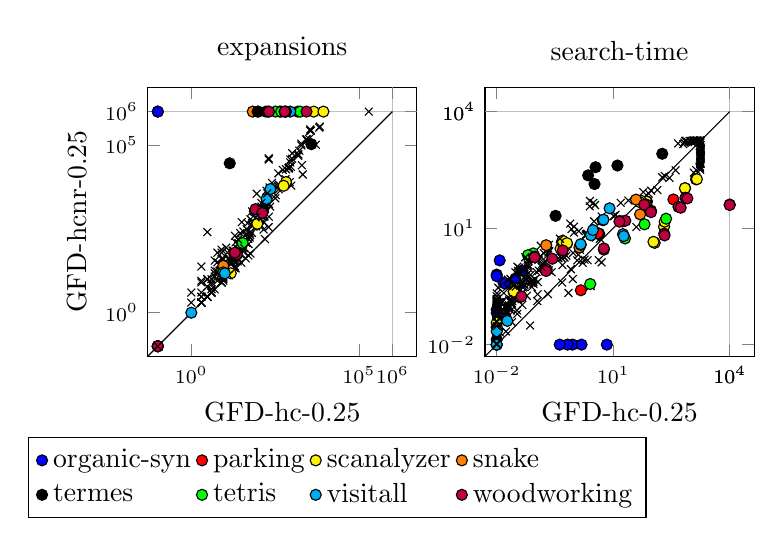
\begin{tikzpicture}
\begin{axis}[at={(0,0)}, extra x tick style={grid=major}, extra x ticks=1000000, extra y tick style={grid=major}, extra y ticks=1000000, height=5cm, legend cell align=left, legend style={at={(1.0, -0.5)}}, title=expansions, width=5cm, xlabel=GFD-hc-0.25, xmin=0.05, xmode=log, ylabel=GFD-hcnr-0.25, ymin=0.05, ymode=log]

\addplot[color=black, mark=x, mark options={{draw=black}}, only marks, forget plot] coordinates {
(202, 357) (0.100000, 0.100000) (157, 157) (42, 42)
};
%\addlegendentry{airport}
\addplot[color=cyan, mark=x, mark options={{draw=black}}, only marks, forget plot] coordinates {
(23, 84) (34, 84)
};
%\addlegendentry{barman}
\addplot[color=magenta, mark=x, mark options={{draw=black}}, only marks, forget plot] coordinates {
(216, 5449) (139, 1000000) (0.100000, 0.100000) (158, 1230) (3, 3) (36, 264) (18, 56) (3, 10) (32, 504) (17, 62) (6, 32) (1, 1) (40, 136) (12, 62) (19, 22) (2, 2) (6, 17) (473, 1000000) (65, 1056) (9, 12)
};
%\addlegendentry{blocks}
\addplot[color=red, mark=x, mark options={{draw=black}}, only marks, forget plot] coordinates {
(35, 88) (0.100000, 0.100000) (15, 35) (11, 87) (41, 203) (13, 42)
};
%\addlegendentry{depot}
\addplot[color=yellow, mark=x, mark options={{draw=black}}, only marks, forget plot] coordinates {
(4, 10) (0.100000, 0.100000) (206, 1701) (20, 24) (51, 112) (65, 475) (255, 7472) (26, 40) (8, 8) (20, 198) (143, 304) (78, 480)
};
%\addlegendentry{driverlog}
\addplot[color=cyan, mark=x, mark options={{draw=black}}, only marks, forget plot] coordinates {
(0.100000, 0.100000)
};
%\addlegendentry{freecell}
\addplot[color=magenta, mark=x, mark options={{draw=black}}, only marks, forget plot] coordinates {
(0.100000, 0.100000)
};
%\addlegendentry{grid}
\addplot[color=black, mark=x, mark options={{draw=black}}, only marks, forget plot] coordinates {
(45, 308) (208, 1776) (668, 19057) (0.100000, 0.100000) (1920, 97200)
};
%\addlegendentry{gripper}
\addplot[color=green, mark=x, mark options={{draw=black}}, only marks, forget plot] coordinates {
(0.100000, 0.100000) (4, 4) (8, 8)
};
%\addlegendentry{hiking}
\addplot[color=red, mark=x, mark options={{draw=black}}, only marks, forget plot] coordinates {
(91, 591) (64, 241) (25, 116) (2, 24) (15, 36) (1027, 57316) (818, 20864) (156, 1310) (405, 4822) (15, 30) (9, 11) (1671, 68464) (1, 1) (0.100000, 0.100000) (26, 116) (9, 20) (535, 18210) (320, 2596) (226, 1464) (36, 129) (133, 740) (14, 16) (175, 4388) (19, 52)
};
%\addlegendentry{logistics}
\addplot[color=black, mark=x, mark options={{draw=black}}, only marks, forget plot] coordinates {
(819, 21330) (14, 37) (18, 37) (57, 211) (395, 5949) (1545, 47759) (166, 1634) (156, 1401) (3709, 271472) (416, 6433) (1019, 39297) (67, 396) (1542, 53181) (164, 1672) (2684, 147165) (330, 3216) (18, 71) (135, 880) (931, 22717) (6534, 333019) (4451, 1000000) (3510, 268001) (409, 6563) (1, 1) (3558, 293838) (824, 21385) (1563, 52503) (649, 9632) (0.100000, 0.100000) (55, 176) (155, 1555) (122, 747) (1908, 110504) (65, 395) (801, 20737) (2841, 136348) (907, 36976) (803, 20047) (17, 70) (67, 387) (391, 5786) (14, 36) (2768, 149220) (6865, 357205) (3249, 153494) (2, 3) (54, 190)
};
%\addlegendentry{miconic}
\addplot[color=cyan, mark=x, mark options={{draw=black}}, only marks, forget plot] coordinates {
(0.100000, 0.100000)
};
%\addlegendentry{movie}
\addplot[color=yellow, mark=x, mark options={{draw=black}}, only marks, forget plot] coordinates {
(0.100000, 0.100000)
};
%\addlegendentry{mprime}
\addplot[color=blue, mark=x, mark options={{draw=black}}, only marks, forget plot] coordinates {
(0.100000, 0.100000)
};
%\addlegendentry{mystery}
\addplot[color=red, mark=x, mark options={{draw=black}}, only marks, forget plot] coordinates {
(7, 18) (0.100000, 0.100000) (1, 1) (58, 617)
};
%\addlegendentry{nomystery}
\addplot[color=red, mark=x, mark options={{draw=black}}, only marks, forget plot] coordinates {
(204, 37149) (8, 62) (204, 40510) (6, 62)
};
%\addlegendentry{openstacks}
\addplot[color=blue, mark=*, mark options={{draw=black}}, only marks, forget plot] coordinates {
(0.100000, 0.100000) (0.100000, 1000000)
};
%\addlegendentry{organic-synthesis}
\addplot[color=blue, mark=*, mark options={{draw=black}}, only marks, forget plot] coordinates {
(0.100000, 0.100000) (0.100000, 1000000)
};
%\addlegendentry{organic-synthesis-split}
\addplot[color=blue, mark=x, mark options={{draw=black}}, only marks, forget plot] coordinates {
(21, 126) (0.100000, 0.100000)
};
%\addlegendentry{pathways-noneg}
\addplot[color=yellow, mark=x, mark options={{draw=black}}, only marks, forget plot] coordinates {
(6, 9) (0.100000, 0.100000) (3, 3) (9, 21) (2, 2) (9, 9) (9, 10) (11, 21) (25, 40) (1, 1)
};
%\addlegendentry{pipesworld-nt}
\addplot[color=green, mark=x, mark options={{draw=black}}, only marks, forget plot] coordinates {
(2, 8) (0.100000, 0.100000) (3, 3) (5, 5) (1, 1)
};
%\addlegendentry{pipesworld-t}
\addplot[color=green, mark=x, mark options={{draw=black}}, only marks, forget plot] coordinates {
(863, 7878) (29, 56) (4, 8) (2109, 13290) (55, 244) (8, 40) (9, 18) (173, 2644) (5183, 102720) (1, 2) (5, 36) (3, 3) (2, 9) (8, 76) (3, 10) (16, 29) (5, 12) (3, 6) (2, 2) (7, 28) (206, 727) (0.100000, 0.100000) (902, 30464) (25, 76) (29, 236) (5, 15) (2, 3) (116, 371) (19, 42) (151, 749) (50, 161) (9, 39) (31, 156) (149, 498) (85, 375) (196523, 1000000) (2, 4) (151, 741) (958, 6186) (9, 40)
};
%\addlegendentry{psr-small}
\addplot[color=black, mark=x, mark options={{draw=black}}, only marks, forget plot] coordinates {
(112, 430) (43, 122) (0.100000, 0.100000) (9, 12) (1997, 25113)
};
%\addlegendentry{rovers}
\addplot[color=blue, mark=x, mark options={{draw=black}}, only marks, forget plot] coordinates {
(0.100000, 0.100000) (1, 1) (89, 3559) (3, 255) (2, 2) (48, 466)
};
%\addlegendentry{satellite}
\addplot[color=yellow, mark=*, mark options={{draw=black}}, only marks, forget plot] coordinates {
(668, 7908) (4471, 1000000) (93, 448) (568, 6122) (0.100000, 0.100000) (8748, 1000000) (15, 15)
};
%\addlegendentry{scanalyzer}
\addplot[color=orange, mark=*, mark options={{draw=black}}, only marks, forget plot] coordinates {
(436, 1000000) (9, 25) (68, 1000000) (168, 1000000)
};
%\addlegendentry{snake}
\addplot[color=magenta, mark=x, mark options={{draw=black}}, only marks, forget plot] coordinates {
(0.100000, 0.100000) (24, 34) (35, 67)
};
%\addlegendentry{storage}
\addplot[color=black, mark=*, mark options={{draw=black}}, only marks, forget plot] coordinates {
(95, 1000000) (99, 1000000) (14, 28672) (193, 1000000) (3812, 106752) (1504, 1000000)
};
%\addlegendentry{termes}
\addplot[color=green, mark=*, mark options={{draw=black}}, only marks, forget plot] coordinates {
(34, 120) (325, 1000000) (480, 1000000) (9, 16) (1776, 1000000)
};
%\addlegendentry{tetris}
\addplot[color=green, mark=x, mark options={{draw=black}}, only marks, forget plot] coordinates {
(4, 7) (7, 13) (3, 3) (4, 4) (0.100000, 0.100000) (1, 1)
};
%\addlegendentry{tidybot}
\addplot[color=red, mark=x, mark options={{draw=black}}, only marks, forget plot] coordinates {
(25, 154) (0.100000, 0.100000) (123, 1478)
};
%\addlegendentry{tpp}
\addplot[color=red, mark=x, mark options={{draw=black}}, only marks, forget plot] coordinates {
(0.100000, 0.100000) (13, 13) (58, 58) (4, 5) (5, 18) (38, 84) (50, 51) (25, 40) (31, 31) (21, 21)
};
%\addlegendentry{transport}
\addplot[color=blue, mark=x, mark options={{draw=black}}, only marks, forget plot] coordinates {
(0.100000, 0.100000)
};
%\addlegendentry{trucks}
\addplot[color=cyan, mark=*, mark options={{draw=black}}, only marks, forget plot] coordinates {
(893, 1000000) (0.100000, 0.100000) (229, 4901) (670, 1000000) (79, 1059) (10, 15) (176, 2486) (1, 1)
};
%\addlegendentry{visitall}
\addplot[color=purple, mark=*, mark options={{draw=black}}, only marks, forget plot] coordinates {
(82, 1229) (0.100000, 0.100000) (131, 940) (23, 55) (617, 1000000) (208, 1000000) (2738, 1000000) (20, 62) (608, 1000000)
};
%\addlegendentry{woodworking}
\addplot[color=blue, mark=x, mark options={{draw=black}}, only marks, forget plot] coordinates {
(0.100000, 0.100000) (123, 1874) (4, 4) (394, 14323) (1, 4) (8, 8) (83, 697) (184, 3618)
};
%\addlegendentry{zenotravel}
\addplot[color=black] coordinates {(0.050000, 0.050000) (1000000, 1000000)};
\end{axis}





%search time
\begin{axis}[at={(20,0)}, extra x tick style={grid=major}, extra x ticks=10000, extra y tick style={grid=major}, extra y ticks=10000, height=5cm, legend cell align=left, legend style={at={(0.6, -0.3)}}, title=search-time, width=5cm, xlabel=GFD-hc-0.25, xmin=0.005, xmode=log, ymin=0.005, ymode=log, legend columns=4]

\addplot[color=green, mark=x, mark options={{draw=black}}, only marks, forget plot] coordinates {
(0.112780, 0.198327) (0.010000, 0.019164) (0.010000, 0.018347) (0.010000, 0.010000) (0.811526, 0.878469) (0.010000, 0.017541) (1.392966, 2.744087) (0.018178, 0.064894) (0.492103, 1.114480) (1.187180, 1.480010) (0.010000, 0.038277) (0.010000, 0.129951) (4.580029, 5.330525) (0.010000, 0.091064) (1691.842493, 1322.792929) (0.010000, 0.048113) (0.010000, 0.131445)
};
%\addlegendentry{airport}
\addplot[color=yellow, mark=x, mark options={{draw=black}}, only marks, forget plot] coordinates {
(0.033120, 0.076361) (0.018508, 0.067104) (0.018524, 0.071270) (0.017666, 0.064389)
};
%\addlegendentry{barman}
\addplot[color=black, mark=x, mark options={{draw=black}}, only marks, forget plot] coordinates {
(0.106117, 0.747937) (0.139880, 1.130550) (0.023761, 0.144192) (0.022883, 0.135841) (5.020920, 19.857987) (0.051333, 0.355636) (0.011663, 0.058854) (0.010000, 0.010000) (0.056137, 0.467749) (0.049992, 0.308721) (0.210779, 2.071900) (0.010000, 0.022584) (0.214123, 2.347050) (0.010000, 0.021646) (0.011186, 0.052181) (0.225803, 2.580250) (0.010000, 0.024214) (0.014036, 0.073485) (1.267270, 2.061785) (0.023624, 0.120193)
};
%\addlegendentry{blocks}
\addplot[color=green, mark=x, mark options={{draw=black}}, only marks, forget plot] coordinates {
(0.047089, 0.296653) (0.010074, 0.063875) (0.020327, 0.088525) (0.051365, 0.349580) (0.012141, 0.123813) (0.010000, 0.010000)
};
%\addlegendentry{depot}
\addplot[color=red, mark=x, mark options={{draw=black}}, only marks, forget plot] coordinates {
(0.054591, 0.512738) (0.011820, 0.030213) (0.087964, 0.362773) (0.044791, 0.215811) (0.222812, 3.707570) (0.027948, 0.219084) (0.096936, 0.482844) (0.012750, 0.072234) (0.080414, 0.303832) (0.237527, 1.795440) (0.010000, 0.010000) (0.023106, 0.076168) (0.010000, 0.013002)
};
%\addlegendentry{driverlog}
\addplot[color=blue, mark=x, mark options={{draw=black}}, only marks, forget plot] coordinates {
(1.826977, 1.545542) (0.110795, 0.131787) (0.208937, 0.199343) (0.010000, 0.029874) (2.632227, 0.323642) (0.072462, 0.031164) (4.240369, 1.496790) (0.912273, 0.487512) (1.645699, 1.275004) (0.703899, 0.213877) (0.485120, 0.397746) (5.025293, 1.308984) (2.182068, 1.488412)
};
%\addlegendentry{floortile}
\addplot[color=yellow, mark=x, mark options={{draw=black}}, only marks, forget plot] coordinates {
(0.010000, 0.096289) (0.010000, 0.014482) (0.010000, 0.123179) (0.010000, 0.135099) (0.010000, 0.139748) (0.010000, 0.149630) (0.010000, 0.103611) (0.010000, 0.084542) (0.010000, 0.084437) (0.010000, 0.054917) (0.010000, 0.068708) (0.010000, 0.030907) (0.010000, 0.095698) (0.010000, 0.130291) (0.010000, 0.072304)
};
%\addlegendentry{freecell}
\addplot[color=black, mark=x, mark options={{draw=black}}, only marks, forget plot] coordinates {
(0.010000, 0.045548) (0.010000, 0.010000)
};
%\addlegendentry{grid}
\addplot[color=green, mark=x, mark options={{draw=black}}, only marks, forget plot] coordinates {
(3.613340, 5.745380) (0.114229, 0.410417) (69.428800, 40.124500) (1683.969572, 374.027407) (1731.840130, 675.209617) (0.010000, 0.010000) (0.010002, 0.043612)
};
%\addlegendentry{gripper}
\addplot[color=green, mark=x, mark options={{draw=black}}, only marks, forget plot] coordinates {
(0.010000, 0.010240) (0.017259, 0.021861) (0.010000, 0.010000)
};
%\addlegendentry{hiking}
\addplot[color=red, mark=x, mark options={{draw=black}}, only marks, forget plot] coordinates {
(0.010000, 0.015940) (0.842363, 9.437350) (2.520830, 49.982100) (0.087762, 0.401981) (0.010000, 0.030010) (0.024731, 0.115098) (2.491980, 36.400500) (0.010000, 0.010000) (0.036979, 0.278576) (0.975676, 10.958800) (0.010000, 0.016523) (0.042243, 0.369600) (0.088012, 0.453266) (0.010000, 0.029815) (0.119733, 1.526640) (0.010000, 0.018769) (0.218992, 0.812916) (0.389319, 1.670570) (0.056266, 0.609610)
};
%\addlegendentry{logistics}
\addplot[color=red, mark=x, mark options={{draw=black}}, only marks, forget plot] coordinates {
(1758.454883, 451.723072) (1784.555846, 625.046578) (1783.392960, 612.141613) (1739.302574, 315.409800) (1396.936730, 1790.859860) (0.020543, 0.102587) (1343.458600, 1780.345654) (1214.667700, 1785.381126) (1774.367246, 832.812426) (1236.519400, 1790.911845) (1695.170330, 1755.414627) (1457.695990, 1784.833575) (95.121600, 92.007100) (1773.630863, 714.656261) (0.010000, 0.024856) (0.080417, 0.431161) (1797.424218, 1073.010056) (0.019771, 0.087963) (1742.421455, 516.392804) (3.643930, 7.914840) (1766.092324, 684.277191) (0.010000, 0.010000) (0.556232, 1.753830) (59.216700, 84.367300) (1770.699554, 813.426270) (280.593000, 196.950000) (1762.724350, 1787.997528) (0.043562, 0.203888) (1776.515704, 933.195019) (0.010000, 0.010201) (0.010905, 0.039571) (0.024835, 0.105955) (0.462530, 1.714130) (2.002460, 6.883860) (0.624117, 1.953380) (24.527300, 51.269600) (137.616000, 95.702500) (1124.430200, 1771.940824) (1755.182973, 480.461774) (0.924303, 2.292340) (0.035658, 0.144173) (1777.739008, 1103.700284) (1754.296950, 620.511863) (4.916260, 14.665700) (2.071620, 6.913400) (1701.857381, 351.829898) (1664.944000, 1790.999986) (1775.961989, 917.895716) (82.159600, 77.440900) (1794.476710, 924.925172) (932.102000, 1765.103581) (0.258800, 0.731319) (1699.198990, 1794.052392) (1715.118656, 376.513908) (1188.980000, 267.526000) (213.320000, 220.455000) (718.532000, 1757.711340) (1.960510, 6.443440) (468.933000, 1516.887500) (183.425000, 203.693000) (1019.232360, 1743.105223) (0.082211, 0.432722) (1081.028100, 1595.900487) (1422.482990, 1784.569563) (1695.700665, 388.895828) (1760.736575, 733.573369) (1500.752010, 1793.952733) (1769.068892, 1372.748427) (1756.331027, 588.459928) (1756.100431, 448.431720) (1719.953112, 1632.852946) (1194.710920, 1781.446228) (0.075792, 0.392522) (676.705200, 1594.288800) (752.554100, 1772.233910) (10.288000, 20.457500) (1770.825585, 745.939521) (841.482000, 1646.701430) (2.151310, 7.150320) (1749.611400, 1794.006577) (1755.994730, 1381.614395) (0.010000, 0.023664) (1310.406500, 1754.296822) (405.371000, 308.579608) (3.208340, 14.979600) (636.977000, 1451.813900) (1379.830000, 311.706000) (1740.428873, 1671.795711) (0.010853, 0.037363) (1705.725876, 350.332301) (1769.663575, 785.902173) (1794.507620, 1043.371432) (0.083866, 0.434201) (1207.112010, 1783.736598) (0.010686, 0.037065) (0.515280, 1.878000) (1737.569132, 1532.739509) (1379.558400, 1767.764765) (10.637500, 20.334200) (11.487900, 22.044000) (1761.070289, 1141.787992)
};
%\addlegendentry{miconic}

\addplot[color=black, mark=x, mark options={{draw=black}}, only marks, forget plot] coordinates {
(0.010000, 0.050826) (0.010000, 0.035596) (0.010000, 0.016542) (0.010000, 0.020320) (0.010000, 0.011074) (0.010000, 0.021827) (0.010000, 0.028115) (0.010000, 0.010000) (0.010000, 0.010863) (0.010000, 0.019874) (0.010000, 0.012505)
};
%\addlegendentry{mprime}
\addplot[color=magenta, mark=x, mark options={{draw=black}}, only marks, forget plot] coordinates {
(0.010000, 0.042143) (0.010000, 0.086483) (0.010000, 0.041073) (0.010000, 0.016675) (0.010000, 0.052047) (0.010000, 0.010000) (0.010000, 0.026462) (0.010000, 0.017516) (0.010000, 0.013411)
};
%\addlegendentry{mystery}
\addplot[color=blue, mark=x, mark options={{draw=black}}, only marks, forget plot] coordinates {
(0.033859, 0.061799) (0.010000, 0.011833) (0.010000, 0.020266) (0.010000, 0.016874) (0.164108, 2.244940) (0.010000, 0.029445) (0.011152, 0.125176) (0.010000, 0.010000) (0.024699, 0.037792) (0.133764, 1.914530) (0.010000, 0.080387)
};
%\addlegendentry{nomystery}
\addplot[color=blue, mark=x, mark options={{draw=black}}, only marks, forget plot] coordinates {
(0.010000, 0.020682) (0.010000, 0.023188) (0.010000, 0.021022) (0.010000, 0.020747) (3.087890, 45.054300) (0.010000, 0.022248) (3.391240, 39.355500)
};
%\addlegendentry{openstacks}


\addplot[color=blue, mark=*, mark options={{draw=black}}, only marks] coordinates {
(0.010000, 0.079843) (0.011918, 1.476270) (0.010000, 0.065329) (0.898165, 0.010000) (0.010000, 0.635602) (0.010000, 0.010000) (0.010000, 0.578103)
};
\addlegendentry{organic-syn}

\addplot[color=blue, mark=*, mark options={{draw=black}}, only marks, forget plot] coordinates {
(1.529610, 0.010000) (6.852800, 0.010000) (0.665566, 0.010000) (0.015000, 0.387728) (0.030260, 0.501791) (0.046129, 0.799463) (0.010000, 0.013611) (0.418922, 0.010000) (0.080380, 1.797640) (0.016974, 0.375984)
};
%\addlegendentry{organic-synthesis-split}

\addplot[color=red, mark=*, mark options={{draw=black}}, only marks] coordinates {
(354.308000, 54.747826) (4.369680, 7.156315) (4.158310, 7.071952) (1.467470, 0.250811) (4.034000, 7.362436)
};
\addlegendentry{parking}



\addplot[color=magenta, mark=x, mark options={{draw=black}}, only marks, forget plot] coordinates {
(0.025173, 0.131342) (0.010000, 0.010000)
};
%\addlegendentry{pathways-noneg}
\addplot[color=red, mark=x, mark options={{draw=black}}, only marks, forget plot] coordinates {
(0.010029, 0.060251) (0.015292, 0.212873) (0.010000, 0.022947) (0.011442, 0.087135) (0.010000, 0.018068) (0.010000, 0.031865) (0.010000, 0.020019) (0.010000, 0.010141) (0.010000, 0.011517) (0.058710, 0.616928) (0.010000, 0.040296) (0.010000, 0.010000) (0.010000, 0.077459) (0.013224, 0.116769) (0.016760, 0.055870) (0.010000, 0.112948)
};
%\addlegendentry{pipesworld-nt}
\addplot[color=cyan, mark=x, mark options={{draw=black}}, only marks, forget plot] coordinates {
(0.010000, 0.054725) (0.010000, 0.121619) (0.018624, 0.309852) (0.010000, 0.208573) (0.010000, 0.013535) (0.010000, 0.031144) (0.010000, 0.010000) (0.010000, 0.027756) (0.010000, 0.082473) (0.010000, 0.105976) (0.037226, 0.948894)
};
%\addlegendentry{pipesworld-t}
\addplot[color=cyan, mark=x, mark options={{draw=black}}, only marks, forget plot] coordinates {
(0.167634, 1.259400) (0.016539, 0.090135) (0.010000, 0.025280) (0.076559, 0.428527) (0.016052, 0.051106) (0.013182, 0.049950) (0.010000, 0.010204) (0.020196, 0.092624) (0.782098, 13.053100) (0.010000, 0.030015) (0.010000, 0.041169) (0.010000, 0.018507) (0.173249, 1.404480) (0.010000, 0.010665) (71.364600, 41.776722) (0.010000, 0.022326) (1.298010, 8.390570) (0.016500, 0.097702) (0.010000, 0.017507) (0.010993, 0.042908) (0.121458, 0.800345) (0.059695, 0.180480) (0.010000, 0.010294) (0.010000, 0.010000)
};
%\addlegendentry{psr-small}
\addplot[color=red, mark=x, mark options={{draw=black}}, only marks, forget plot] coordinates {
(0.045690, 0.105527) (0.020222, 0.055336) (0.010000, 0.025106) (39.464200, 10.708100) (0.010000, 0.010000)
};
%\addlegendentry{rovers}
\addplot[color=blue, mark=x, mark options={{draw=black}}, only marks, forget plot] coordinates {
(0.020869, 0.137167) (0.031974, 0.282129) (0.135445, 3.531220) (0.021938, 0.092936) (0.010000, 0.010000)
};
%\addlegendentry{satellite}
\addplot[color=yellow, mark=*, mark options={{draw=black}}, only marks] coordinates {
(203.426453, 10.813615) (74.017800, 48.652022) (211.909232, 14.681458) (0.028347, 0.222258) (116.788644, 4.171740) (1355.398989, 180.049969) (0.027595, 0.227983) (0.643558, 3.985290) (71.621600, 48.346642) (0.027768, 0.217251) (708.724017, 106.487008) (51.352900, 51.223346) (108.806030, 4.432177) (0.440953, 2.915580) (47.885800, 46.914166) (0.027464, 0.232904) (0.479151, 4.401790) (0.010000, 0.028035) (703.002174, 106.674992) (1427.805137, 181.877305) (0.495834, 4.737220) (0.645675, 4.098930) (0.010000, 0.036820)
};
\addlegendentry{scanalyzer}
\addplot[color=orange, mark=*, mark options={{draw=black}}, only marks] coordinates {
(38.648530, 54.249486) (49.235100, 22.591818) (0.187869, 3.629110) (0.010000, 0.010000) (1.347050, 3.183905) (1.458500, 3.711125)
};
\addlegendentry{snake}
\addplot[color=yellow, mark=x, mark options={{draw=black}}, only marks, forget plot] coordinates {
(0.010000, 0.023979) (0.010000, 0.023523) (0.019200, 0.095873) (0.011441, 0.030044) (0.010000, 0.010000) (0.010000, 0.040493)
};
%\addlegendentry{storage}
\addplot[color=black, mark=*, mark options={{draw=black}}, only marks] coordinates {
(0.327863, 20.734600) (183.306000, 821.597441) (3.508920, 369.800274) (3.310920, 136.234000) (2.260760, 228.032686) (12.841000, 409.058131)
};
\addlegendentry{termes}
\addplot[color=green, mark=*, mark options={{draw=black}}, only marks] coordinates {
(0.087094, 2.231570) (2.559430, 0.363580) (20.143500, 5.420359) (0.063869, 2.008870) (63.796000, 12.543131) (230.241303, 17.483130)
};
\addlegendentry{tetris}
\addplot[color=blue, mark=x, mark options={{draw=black}}, only marks, forget plot] coordinates {
(0.019319, 0.473506) (0.042040, 0.648883) (0.027109, 0.323255) (0.037462, 0.723225) (0.035466, 0.786945) (0.065097, 1.070840) (0.030351, 0.729299) (0.080278, 1.611100) (0.022600, 0.489540) (0.054421, 1.780740) (0.066010, 0.931967) (0.033915, 1.014210) (0.065018, 1.382880) (0.038939, 0.726956) (0.026864, 0.358107) (0.050462, 0.854148) (0.073953, 0.623370) (0.010000, 0.175639) (0.042476, 0.448563) (0.103977, 1.592870) (0.010952, 0.290943) (0.062857, 1.160410) (0.062862, 1.537910)
};
%\addlegendentry{tidybot}
\addplot[color=blue, mark=x, mark options={{draw=black}}, only marks, forget plot] coordinates {
(0.010000, 0.010000) (0.010000, 0.052804) (0.046523, 0.369383)
};
%\addlegendentry{tpp}
\addplot[color=green, mark=x, mark options={{draw=black}}, only marks, forget plot] coordinates {
(0.010000, 0.023169) (0.010000, 0.064205) (0.029663, 0.147973) (0.010000, 0.038112) (0.010000, 0.010672) (0.010000, 0.010000) (0.010000, 0.039217) (0.012020, 0.020608) (0.010000, 0.059111) (0.010000, 0.021860) (0.010000, 0.057709) (0.010000, 0.017416) (0.010000, 0.011923) (0.010000, 0.014073) (0.010000, 0.028013) (0.010000, 0.012332)
};
%\addlegendentry{transport}
\addplot[color=magenta, mark=x, mark options={{draw=black}}, only marks, forget plot] coordinates {
(0.010000, 0.010000)
};
%\addlegendentry{trucks}
\addplot[color=cyan, mark=*, mark options={{draw=black}}, only marks] coordinates {
(17.853300, 6.986764) (5.372019, 15.997092) (1.451020, 3.850950) (2.658960, 6.552700) (8.048821, 32.363919) (5.617487, 16.460272) (3.008980, 8.905630) (0.010000, 0.010000) (0.010000, 0.021872) (0.018731, 0.040848) (18.687500, 6.229438)
};
\addlegendentry{visitall}
\addplot[color=purple, mark=*, mark options={{draw=black}}, only marks] coordinates {
(205.160000, 7.237639) (723.500819, 60.597384) (0.270261, 1.627080) (478.960000, 35.206969) (71.184424, 40.509067) (14.716000, 15.257454) (17.274288, 14.872363) (10000, 40.471993) (5.732910, 2.777757) (0.095040, 1.835804) (812.101823, 58.104613) (0.193118, 0.870327) (0.185642, 0.785668) (20.525555, 15.476348) (0.043164, 0.173316) (210.175000, 6.488662) (0.094698, 1.770294) (93.950510, 28.189315) (5.738660, 3.002524) (62.870901, 39.979857) (94.167276, 25.744202) (546.009000, 33.469259) (0.502560, 2.670380) (14.487000, 14.666541) (10000, 39.328732)
};
\addlegendentry{woodworking}
\addplot[color=cyan, mark=x, mark options={{draw=black}}, only marks, forget plot] coordinates {
(15.639000, 44.734700) (0.010000, 0.014936) (0.426344, 5.324050) (0.978021, 7.639780) (0.010000, 0.029947) (0.010000, 0.010488) (0.030934, 0.310911) (0.010000, 0.010000) (0.014032, 0.132001) (0.010000, 0.010557) (0.141588, 1.013860)
};
%\addlegendentry{zenotravel}
\addplot[color=black] coordinates {(0.0050000, 0.0050000) (10000, 10000)};
\end{axis}
\end{tikzpicture}
	\end{minipage}
	%\hfill
	%\begin{minipage}{0.2\textwidth}
	%	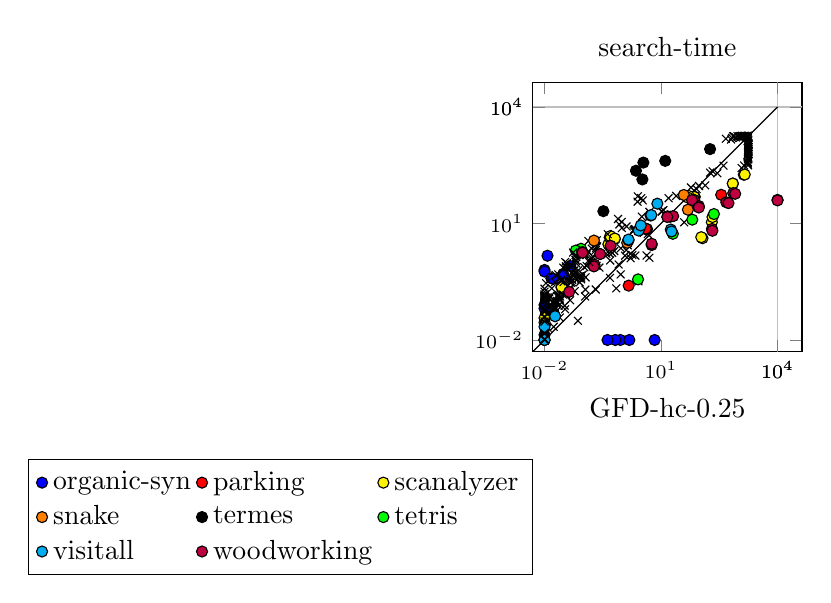
\begin{tikzpicture}
\begin{axis}[extra x tick style={grid=major}, extra x ticks=10000, extra y tick style={grid=major}, extra y ticks=10000, height=5cm, legend cell align=left, legend style={at={(0.0, -0.4)}}, title=search-time, width=5cm, xlabel=GFD-hc-0.25, xmin=0.005, xmode=log, ymin=0.005, ymode=log, legend columns=3]

\addplot[color=green, mark=x, mark options={{draw=black}}, only marks, forget plot] coordinates {
(0.112780, 0.198327) (0.010000, 0.019164) (0.010000, 0.018347) (0.010000, 0.010000) (0.811526, 0.878469) (0.010000, 0.017541) (1.392966, 2.744087) (0.018178, 0.064894) (0.492103, 1.114480) (1.187180, 1.480010) (0.010000, 0.038277) (0.010000, 0.129951) (4.580029, 5.330525) (0.010000, 0.091064) (1691.842493, 1322.792929) (0.010000, 0.048113) (0.010000, 0.131445)
};
%\addlegendentry{airport}
\addplot[color=yellow, mark=x, mark options={{draw=black}}, only marks, forget plot] coordinates {
(0.033120, 0.076361) (0.018508, 0.067104) (0.018524, 0.071270) (0.017666, 0.064389)
};
%\addlegendentry{barman}
\addplot[color=black, mark=x, mark options={{draw=black}}, only marks, forget plot] coordinates {
(0.106117, 0.747937) (0.139880, 1.130550) (0.023761, 0.144192) (0.022883, 0.135841) (5.020920, 19.857987) (0.051333, 0.355636) (0.011663, 0.058854) (0.010000, 0.010000) (0.056137, 0.467749) (0.049992, 0.308721) (0.210779, 2.071900) (0.010000, 0.022584) (0.214123, 2.347050) (0.010000, 0.021646) (0.011186, 0.052181) (0.225803, 2.580250) (0.010000, 0.024214) (0.014036, 0.073485) (1.267270, 2.061785) (0.023624, 0.120193)
};
%\addlegendentry{blocks}
\addplot[color=green, mark=x, mark options={{draw=black}}, only marks, forget plot] coordinates {
(0.047089, 0.296653) (0.010074, 0.063875) (0.020327, 0.088525) (0.051365, 0.349580) (0.012141, 0.123813) (0.010000, 0.010000)
};
%\addlegendentry{depot}
\addplot[color=red, mark=x, mark options={{draw=black}}, only marks, forget plot] coordinates {
(0.054591, 0.512738) (0.011820, 0.030213) (0.087964, 0.362773) (0.044791, 0.215811) (0.222812, 3.707570) (0.027948, 0.219084) (0.096936, 0.482844) (0.012750, 0.072234) (0.080414, 0.303832) (0.237527, 1.795440) (0.010000, 0.010000) (0.023106, 0.076168) (0.010000, 0.013002)
};
%\addlegendentry{driverlog}
\addplot[color=blue, mark=x, mark options={{draw=black}}, only marks, forget plot] coordinates {
(1.826977, 1.545542) (0.110795, 0.131787) (0.208937, 0.199343) (0.010000, 0.029874) (2.632227, 0.323642) (0.072462, 0.031164) (4.240369, 1.496790) (0.912273, 0.487512) (1.645699, 1.275004) (0.703899, 0.213877) (0.485120, 0.397746) (5.025293, 1.308984) (2.182068, 1.488412)
};
%\addlegendentry{floortile}
\addplot[color=yellow, mark=x, mark options={{draw=black}}, only marks, forget plot] coordinates {
(0.010000, 0.096289) (0.010000, 0.014482) (0.010000, 0.123179) (0.010000, 0.135099) (0.010000, 0.139748) (0.010000, 0.149630) (0.010000, 0.103611) (0.010000, 0.084542) (0.010000, 0.084437) (0.010000, 0.054917) (0.010000, 0.068708) (0.010000, 0.030907) (0.010000, 0.095698) (0.010000, 0.130291) (0.010000, 0.072304)
};
%\addlegendentry{freecell}
\addplot[color=black, mark=x, mark options={{draw=black}}, only marks, forget plot] coordinates {
(0.010000, 0.045548) (0.010000, 0.010000)
};
%\addlegendentry{grid}
\addplot[color=green, mark=x, mark options={{draw=black}}, only marks, forget plot] coordinates {
(3.613340, 5.745380) (0.114229, 0.410417) (69.428800, 40.124500) (1683.969572, 374.027407) (1731.840130, 675.209617) (0.010000, 0.010000) (0.010002, 0.043612)
};
%\addlegendentry{gripper}
\addplot[color=green, mark=x, mark options={{draw=black}}, only marks, forget plot] coordinates {
(0.010000, 0.010240) (0.017259, 0.021861) (0.010000, 0.010000)
};
%\addlegendentry{hiking}
\addplot[color=red, mark=x, mark options={{draw=black}}, only marks, forget plot] coordinates {
(0.010000, 0.015940) (0.842363, 9.437350) (2.520830, 49.982100) (0.087762, 0.401981) (0.010000, 0.030010) (0.024731, 0.115098) (2.491980, 36.400500) (0.010000, 0.010000) (0.036979, 0.278576) (0.975676, 10.958800) (0.010000, 0.016523) (0.042243, 0.369600) (0.088012, 0.453266) (0.010000, 0.029815) (0.119733, 1.526640) (0.010000, 0.018769) (0.218992, 0.812916) (0.389319, 1.670570) (0.056266, 0.609610)
};
%\addlegendentry{logistics}
\addplot[color=red, mark=x, mark options={{draw=black}}, only marks, forget plot] coordinates {
(1758.454883, 451.723072) (1784.555846, 625.046578) (1783.392960, 612.141613) (1739.302574, 315.409800) (1396.936730, 1790.859860) (0.020543, 0.102587) (1343.458600, 1780.345654) (1214.667700, 1785.381126) (1774.367246, 832.812426) (1236.519400, 1790.911845) (1695.170330, 1755.414627) (1457.695990, 1784.833575) (95.121600, 92.007100) (1773.630863, 714.656261) (0.010000, 0.024856) (0.080417, 0.431161) (1797.424218, 1073.010056) (0.019771, 0.087963) (1742.421455, 516.392804) (3.643930, 7.914840) (1766.092324, 684.277191) (0.010000, 0.010000) (0.556232, 1.753830) (59.216700, 84.367300) (1770.699554, 813.426270) (280.593000, 196.950000) (1762.724350, 1787.997528) (0.043562, 0.203888) (1776.515704, 933.195019) (0.010000, 0.010201) (0.010905, 0.039571) (0.024835, 0.105955) (0.462530, 1.714130) (2.002460, 6.883860) (0.624117, 1.953380) (24.527300, 51.269600) (137.616000, 95.702500) (1124.430200, 1771.940824) (1755.182973, 480.461774) (0.924303, 2.292340) (0.035658, 0.144173) (1777.739008, 1103.700284) (1754.296950, 620.511863) (4.916260, 14.665700) (2.071620, 6.913400) (1701.857381, 351.829898) (1664.944000, 1790.999986) (1775.961989, 917.895716) (82.159600, 77.440900) (1794.476710, 924.925172) (932.102000, 1765.103581) (0.258800, 0.731319) (1699.198990, 1794.052392) (1715.118656, 376.513908) (1188.980000, 267.526000) (213.320000, 220.455000) (718.532000, 1757.711340) (1.960510, 6.443440) (468.933000, 1516.887500) (183.425000, 203.693000) (1019.232360, 1743.105223) (0.082211, 0.432722) (1081.028100, 1595.900487) (1422.482990, 1784.569563) (1695.700665, 388.895828) (1760.736575, 733.573369) (1500.752010, 1793.952733) (1769.068892, 1372.748427) (1756.331027, 588.459928) (1756.100431, 448.431720) (1719.953112, 1632.852946) (1194.710920, 1781.446228) (0.075792, 0.392522) (676.705200, 1594.288800) (752.554100, 1772.233910) (10.288000, 20.457500) (1770.825585, 745.939521) (841.482000, 1646.701430) (2.151310, 7.150320) (1749.611400, 1794.006577) (1755.994730, 1381.614395) (0.010000, 0.023664) (1310.406500, 1754.296822) (405.371000, 308.579608) (3.208340, 14.979600) (636.977000, 1451.813900) (1379.830000, 311.706000) (1740.428873, 1671.795711) (0.010853, 0.037363) (1705.725876, 350.332301) (1769.663575, 785.902173) (1794.507620, 1043.371432) (0.083866, 0.434201) (1207.112010, 1783.736598) (0.010686, 0.037065) (0.515280, 1.878000) (1737.569132, 1532.739509) (1379.558400, 1767.764765) (10.637500, 20.334200) (11.487900, 22.044000) (1761.070289, 1141.787992)
};
%\addlegendentry{miconic}

\addplot[color=black, mark=x, mark options={{draw=black}}, only marks, forget plot] coordinates {
(0.010000, 0.050826) (0.010000, 0.035596) (0.010000, 0.016542) (0.010000, 0.020320) (0.010000, 0.011074) (0.010000, 0.021827) (0.010000, 0.028115) (0.010000, 0.010000) (0.010000, 0.010863) (0.010000, 0.019874) (0.010000, 0.012505)
};
%\addlegendentry{mprime}
\addplot[color=magenta, mark=x, mark options={{draw=black}}, only marks, forget plot] coordinates {
(0.010000, 0.042143) (0.010000, 0.086483) (0.010000, 0.041073) (0.010000, 0.016675) (0.010000, 0.052047) (0.010000, 0.010000) (0.010000, 0.026462) (0.010000, 0.017516) (0.010000, 0.013411)
};
%\addlegendentry{mystery}
\addplot[color=blue, mark=x, mark options={{draw=black}}, only marks, forget plot] coordinates {
(0.033859, 0.061799) (0.010000, 0.011833) (0.010000, 0.020266) (0.010000, 0.016874) (0.164108, 2.244940) (0.010000, 0.029445) (0.011152, 0.125176) (0.010000, 0.010000) (0.024699, 0.037792) (0.133764, 1.914530) (0.010000, 0.080387)
};
%\addlegendentry{nomystery}
\addplot[color=blue, mark=x, mark options={{draw=black}}, only marks, forget plot] coordinates {
(0.010000, 0.020682) (0.010000, 0.023188) (0.010000, 0.021022) (0.010000, 0.020747) (3.087890, 45.054300) (0.010000, 0.022248) (3.391240, 39.355500)
};
%\addlegendentry{openstacks}


\addplot[color=blue, mark=*, mark options={{draw=black}}, only marks] coordinates {
(0.010000, 0.079843) (0.011918, 1.476270) (0.010000, 0.065329) (0.898165, 0.010000) (0.010000, 0.635602) (0.010000, 0.010000) (0.010000, 0.578103)
};
\addlegendentry{organic-syn}

\addplot[color=blue, mark=*, mark options={{draw=black}}, only marks, forget plot] coordinates {
(1.529610, 0.010000) (6.852800, 0.010000) (0.665566, 0.010000) (0.015000, 0.387728) (0.030260, 0.501791) (0.046129, 0.799463) (0.010000, 0.013611) (0.418922, 0.010000) (0.080380, 1.797640) (0.016974, 0.375984)
};
%\addlegendentry{organic-synthesis-split}

\addplot[color=red, mark=*, mark options={{draw=black}}, only marks] coordinates {
(354.308000, 54.747826) (4.369680, 7.156315) (4.158310, 7.071952) (1.467470, 0.250811) (4.034000, 7.362436)
};
\addlegendentry{parking}



\addplot[color=magenta, mark=x, mark options={{draw=black}}, only marks, forget plot] coordinates {
(0.025173, 0.131342) (0.010000, 0.010000)
};
%\addlegendentry{pathways-noneg}
\addplot[color=red, mark=x, mark options={{draw=black}}, only marks, forget plot] coordinates {
(0.010029, 0.060251) (0.015292, 0.212873) (0.010000, 0.022947) (0.011442, 0.087135) (0.010000, 0.018068) (0.010000, 0.031865) (0.010000, 0.020019) (0.010000, 0.010141) (0.010000, 0.011517) (0.058710, 0.616928) (0.010000, 0.040296) (0.010000, 0.010000) (0.010000, 0.077459) (0.013224, 0.116769) (0.016760, 0.055870) (0.010000, 0.112948)
};
%\addlegendentry{pipesworld-nt}
\addplot[color=cyan, mark=x, mark options={{draw=black}}, only marks, forget plot] coordinates {
(0.010000, 0.054725) (0.010000, 0.121619) (0.018624, 0.309852) (0.010000, 0.208573) (0.010000, 0.013535) (0.010000, 0.031144) (0.010000, 0.010000) (0.010000, 0.027756) (0.010000, 0.082473) (0.010000, 0.105976) (0.037226, 0.948894)
};
%\addlegendentry{pipesworld-t}
\addplot[color=cyan, mark=x, mark options={{draw=black}}, only marks, forget plot] coordinates {
(0.167634, 1.259400) (0.016539, 0.090135) (0.010000, 0.025280) (0.076559, 0.428527) (0.016052, 0.051106) (0.013182, 0.049950) (0.010000, 0.010204) (0.020196, 0.092624) (0.782098, 13.053100) (0.010000, 0.030015) (0.010000, 0.041169) (0.010000, 0.018507) (0.173249, 1.404480) (0.010000, 0.010665) (71.364600, 41.776722) (0.010000, 0.022326) (1.298010, 8.390570) (0.016500, 0.097702) (0.010000, 0.017507) (0.010993, 0.042908) (0.121458, 0.800345) (0.059695, 0.180480) (0.010000, 0.010294) (0.010000, 0.010000)
};
%\addlegendentry{psr-small}
\addplot[color=red, mark=x, mark options={{draw=black}}, only marks, forget plot] coordinates {
(0.045690, 0.105527) (0.020222, 0.055336) (0.010000, 0.025106) (39.464200, 10.708100) (0.010000, 0.010000)
};
%\addlegendentry{rovers}
\addplot[color=blue, mark=x, mark options={{draw=black}}, only marks, forget plot] coordinates {
(0.020869, 0.137167) (0.031974, 0.282129) (0.135445, 3.531220) (0.021938, 0.092936) (0.010000, 0.010000)
};
%\addlegendentry{satellite}
\addplot[color=yellow, mark=*, mark options={{draw=black}}, only marks] coordinates {
(203.426453, 10.813615) (74.017800, 48.652022) (211.909232, 14.681458) (0.028347, 0.222258) (116.788644, 4.171740) (1355.398989, 180.049969) (0.027595, 0.227983) (0.643558, 3.985290) (71.621600, 48.346642) (0.027768, 0.217251) (708.724017, 106.487008) (51.352900, 51.223346) (108.806030, 4.432177) (0.440953, 2.915580) (47.885800, 46.914166) (0.027464, 0.232904) (0.479151, 4.401790) (0.010000, 0.028035) (703.002174, 106.674992) (1427.805137, 181.877305) (0.495834, 4.737220) (0.645675, 4.098930) (0.010000, 0.036820)
};
\addlegendentry{scanalyzer}
\addplot[color=orange, mark=*, mark options={{draw=black}}, only marks] coordinates {
(38.648530, 54.249486) (49.235100, 22.591818) (0.187869, 3.629110) (0.010000, 0.010000) (1.347050, 3.183905) (1.458500, 3.711125)
};
\addlegendentry{snake}
\addplot[color=yellow, mark=x, mark options={{draw=black}}, only marks, forget plot] coordinates {
(0.010000, 0.023979) (0.010000, 0.023523) (0.019200, 0.095873) (0.011441, 0.030044) (0.010000, 0.010000) (0.010000, 0.040493)
};
%\addlegendentry{storage}
\addplot[color=black, mark=*, mark options={{draw=black}}, only marks] coordinates {
(0.327863, 20.734600) (183.306000, 821.597441) (3.508920, 369.800274) (3.310920, 136.234000) (2.260760, 228.032686) (12.841000, 409.058131)
};
\addlegendentry{termes}
\addplot[color=green, mark=*, mark options={{draw=black}}, only marks] coordinates {
(0.087094, 2.231570) (2.559430, 0.363580) (20.143500, 5.420359) (0.063869, 2.008870) (63.796000, 12.543131) (230.241303, 17.483130)
};
\addlegendentry{tetris}
\addplot[color=blue, mark=x, mark options={{draw=black}}, only marks, forget plot] coordinates {
(0.019319, 0.473506) (0.042040, 0.648883) (0.027109, 0.323255) (0.037462, 0.723225) (0.035466, 0.786945) (0.065097, 1.070840) (0.030351, 0.729299) (0.080278, 1.611100) (0.022600, 0.489540) (0.054421, 1.780740) (0.066010, 0.931967) (0.033915, 1.014210) (0.065018, 1.382880) (0.038939, 0.726956) (0.026864, 0.358107) (0.050462, 0.854148) (0.073953, 0.623370) (0.010000, 0.175639) (0.042476, 0.448563) (0.103977, 1.592870) (0.010952, 0.290943) (0.062857, 1.160410) (0.062862, 1.537910)
};
%\addlegendentry{tidybot}
\addplot[color=blue, mark=x, mark options={{draw=black}}, only marks, forget plot] coordinates {
(0.010000, 0.010000) (0.010000, 0.052804) (0.046523, 0.369383)
};
%\addlegendentry{tpp}
\addplot[color=green, mark=x, mark options={{draw=black}}, only marks, forget plot] coordinates {
(0.010000, 0.023169) (0.010000, 0.064205) (0.029663, 0.147973) (0.010000, 0.038112) (0.010000, 0.010672) (0.010000, 0.010000) (0.010000, 0.039217) (0.012020, 0.020608) (0.010000, 0.059111) (0.010000, 0.021860) (0.010000, 0.057709) (0.010000, 0.017416) (0.010000, 0.011923) (0.010000, 0.014073) (0.010000, 0.028013) (0.010000, 0.012332)
};
%\addlegendentry{transport}
\addplot[color=magenta, mark=x, mark options={{draw=black}}, only marks, forget plot] coordinates {
(0.010000, 0.010000)
};
%\addlegendentry{trucks}
\addplot[color=cyan, mark=*, mark options={{draw=black}}, only marks] coordinates {
(17.853300, 6.986764) (5.372019, 15.997092) (1.451020, 3.850950) (2.658960, 6.552700) (8.048821, 32.363919) (5.617487, 16.460272) (3.008980, 8.905630) (0.010000, 0.010000) (0.010000, 0.021872) (0.018731, 0.040848) (18.687500, 6.229438)
};
\addlegendentry{visitall}
\addplot[color=purple, mark=*, mark options={{draw=black}}, only marks] coordinates {
(205.160000, 7.237639) (723.500819, 60.597384) (0.270261, 1.627080) (478.960000, 35.206969) (71.184424, 40.509067) (14.716000, 15.257454) (17.274288, 14.872363) (10000, 40.471993) (5.732910, 2.777757) (0.095040, 1.835804) (812.101823, 58.104613) (0.193118, 0.870327) (0.185642, 0.785668) (20.525555, 15.476348) (0.043164, 0.173316) (210.175000, 6.488662) (0.094698, 1.770294) (93.950510, 28.189315) (5.738660, 3.002524) (62.870901, 39.979857) (94.167276, 25.744202) (546.009000, 33.469259) (0.502560, 2.670380) (14.487000, 14.666541) (10000, 39.328732)
};
\addlegendentry{woodworking}
\addplot[color=cyan, mark=x, mark options={{draw=black}}, only marks, forget plot] coordinates {
(15.639000, 44.734700) (0.010000, 0.014936) (0.426344, 5.324050) (0.978021, 7.639780) (0.010000, 0.029947) (0.010000, 0.010488) (0.030934, 0.310911) (0.010000, 0.010000) (0.014032, 0.132001) (0.010000, 0.010557) (0.141588, 1.013860)
};
%\addlegendentry{zenotravel}
\addplot[color=black] coordinates {(0.0050000, 0.0050000) (10000, 10000)};
\end{axis}
\end{tikzpicture}
	%\end{minipage}
	\begin{minipage}{0.2\textwidth}
		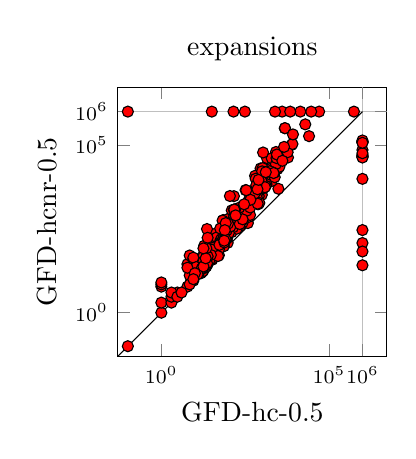
\begin{tikzpicture}
\begin{axis}[extra x tick style={grid=major}, extra x ticks=1000000, extra y tick style={grid=major}, extra y ticks=1000000, height=5cm, legend cell align=left, legend style={at={(1.3, 0.5)}}, title=expansions, width=5cm, xlabel=GFD-hc-0.5, xmin=0.05, xmode=log, ylabel=GFD-hcnr-0.5, ymin=0.05, ymode=log]
\addplot[color=red, mark=*, mark options={{draw=black}}, only marks] coordinates {
(19675, 416544) (3104, 4984) (20, 25) (63, 135) (91, 187) (121, 708) (22, 44) (13, 17) (4338, 58461) (147, 1065) (1, 6) (46, 78) (33, 65) (4955, 60566) (126, 1131) (347, 858) (95, 121) (1794, 19486) (1960, 8490) (4811, 319773) (59, 118) (15, 15) (6, 28) (29, 47) (289, 1470) (1, 1) (1000000, 125176) (70, 580) (1, 2) (32, 63) (391, 1227) (2936, 19354) (311, 1000000) (10, 13) (77, 154) (63, 223) (63, 241) (556807, 1000000) (183, 483) (56, 151) (381, 473) (649, 3465) (19, 60) (401, 720) (543, 4117) (1000000, 44409) (727, 2439) (24, 28) (195, 495) (22, 25) (1000000, 51044) (231, 928) (1069, 4857) (914, 20182) (9, 9) (97, 452) (51, 165) (354, 1334) (91, 164) (4008, 1000000) (50966, 1000000) (60, 115) (2282, 16310) (1000000, 47321) (71, 151) (28, 78) (2408, 11065) (793, 7645) (745, 2688) (16, 16) (160, 597) (55, 186) (1415, 40954) (1000000, 47120) (29498, 1000000) (8, 9) (7, 51) (17, 19) (35, 70) (60, 128) (117, 327) (449, 1726) (22, 24) (40, 227) (146, 3001) (417, 1367) (2896, 27945) (9, 40) (551, 2477) (45, 176) (1000000, 126694) (902, 6275) (17, 24) (84, 156) (43, 88) (23, 314) (2, 2) (144, 435) (179, 481) (242, 619) (987, 15235) (27, 54) (1000000, 120) (52, 52) (73, 96) (100, 316) (15, 25) (18, 18) (39, 78) (213, 931) (1000000, 122229) (12, 18) (33, 38) (1000000, 26) (17, 27) (88, 244) (2726, 58064) (2352, 15271) (2629, 62494) (137, 653) (68, 188) (17, 28) (1366, 6870) (1000000, 9853) (223, 384) (2421, 18135) (19, 100) (992, 3282) (27, 38) (5992, 42714) (1000000, 71893) (56, 99) (73, 139) (167, 592) (1960, 40507) (23, 33) (80, 153) (7560, 100166) (296, 1188) (92, 217) (17, 17) (803, 3022) (32, 1000000) (310, 867) (3331, 22681) (142, 1000000) (272, 1545) (133, 428) (158, 648) (2614, 27214) (396, 2146) (18, 48) (25480, 185128) (17, 22) (764, 1774) (11, 14) (93, 611) (151, 780) (155, 1204) (144, 689) (4881, 320447) (20, 30) (9, 44) (508, 3320) (1000000, 42693) (835, 9442) (1000000, 137745) (125, 253) (111, 3029) (59, 149) (1047, 20567) (1028, 4987) (86, 206) (1017, 5306) (443, 3510) (2159, 15261) (323, 1395) (269, 499) (352, 1385) (213, 657) (1025, 5152) (67, 561) (145, 1188) (1302, 6110) (105, 410) (443, 826) (729, 3670) (20, 22) (33, 64) (2731, 41032) (5860, 61426) (177, 319) (13, 15) (1000000, 67) (8151, 107988) (100, 410) (493, 1916) (876, 5124) (2, 3) (22, 37) (386, 1711) (67, 145) (18, 22) (259, 579) (137, 351) (103, 239) (277, 1161) (90, 288) (7, 13) (1000000, 57496) (2800, 52482) (147, 555) (625, 12152) (408, 1400) (1013, 16508) (57, 325) (92, 423) (3, 4) (2, 4) (432, 2572) (652, 9941) (78, 156) (0.100000, 1000000) (974, 8330) (82, 156) (31, 98) (6, 6) (14022, 1000000) (36, 88) (1233, 5566) (7, 7) (187, 488) (56, 100) (11, 23) (1707, 16634) (2228, 14732) (16, 21) (460, 1675) (521, 2527) (120, 438) (6986, 1000000) (32, 40) (55, 120) (8439, 208722) (12, 14) (52, 77) (723, 2514) (1000000, 292) (765, 1714) (3, 3) (18, 34) (352, 1102) (4, 4) (4084, 34055) (32, 76) (678, 6371) (19, 25) (602, 3537) (6, 22) (212, 1362) (28, 39) (23, 30) (49, 49) (115, 374) (446, 1378) (837, 1886) (0.100000, 0.100000) (737, 4825) (30, 53) (18, 24) (24, 48) (219, 442) (10, 15) (9, 10) (97, 453) (24, 172) (326, 4556) (83, 471) (792, 9194) (746, 1794) (159, 1180) (22, 84) (1084, 60319) (1, 7) (150, 1196) (57, 113) (1304, 15612) (266, 611) (454, 2342) (295, 1720) (340, 4510) (1000000, 117250) (1, 8) (21, 42) (54, 106) (76, 125) (18, 83) (2459, 1000000) (78, 290) (164, 801) (4582, 88624) (75, 141)
};
\addplot[color=black] coordinates {(0.050000, 0.050000) (1000000, 1000000)};
\end{axis}
\end{tikzpicture}
	\end{minipage}
	\hfill
	\begin{minipage}{0.2\textwidth}
		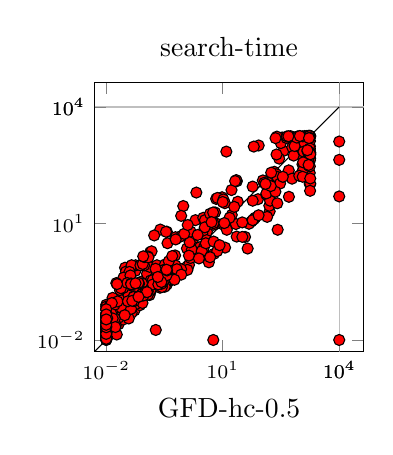
\begin{tikzpicture}
\begin{axis}[extra x tick style={grid=major}, extra x ticks=10000, extra y tick style={grid=major}, extra y ticks=10000, height=5cm, legend cell align=left, legend style={at={(1.3, 0.5)}}, title=search-time, width=5cm, xlabel=GFD-hc-0.5, xmin=0.005, xmode=log, ymin=0.005, ymode=log]
\addplot[color=red, mark=*, mark options={{draw=black}}, only marks] coordinates {
(0.141600, 0.205991) (1605.181010, 1782.630193) (12.400500, 709.237212) (1774.631742, 1791.371591) (212.897000, 213.781000) (1597.457079, 1787.500706) (0.010319, 0.015237) (0.010000, 0.013313) (863.055716, 800.358567) (161.787000, 20.520400) (0.032666, 0.692598) (0.013479, 0.026574) (0.010000, 0.080420) (0.135948, 1.828040) (0.010000, 0.028430) (1.796240, 2.829000) (1.984320, 12.173801) (3.303470, 1.674940) (0.010000, 0.043398) (0.016543, 0.053114) (0.025542, 0.044333) (0.121820, 0.184119) (0.168530, 0.410830) (0.012618, 0.020525) (0.010000, 0.033399) (0.026364, 0.060622) (4.466420, 9.015970) (0.020841, 0.025520) (0.030609, 0.725866) (1.679430, 2.531030) (0.024297, 0.112212) (68.796900, 14.125500) (1.390020, 1.946460) (1776.725506, 100.854000) (0.788609, 4.536800) (0.147242, 1.920020) (0.038869, 0.098166) (0.054435, 0.136739) (0.052649, 0.114803) (10000, 1288.588000) (0.229876, 0.280588) (213.965000, 71.343100) (0.963672, 28.123200) (0.042179, 0.050949) (1035.330000, 1076.700000) (0.010000, 0.013908) (1759.657028, 974.054000) (1.492400, 6.166240) (0.053980, 0.175691) (0.010000, 0.028648) (2.610900, 2.456000) (0.363100, 0.265775) (171.834000, 154.185000) (1748.862219, 437.770512) (0.022541, 0.192919) (1742.277675, 600.521000) (43.841020, 2.263690) (0.053471, 0.057716) (657.472000, 1639.216890) (0.010000, 0.013867) (0.010000, 0.012813) (23.112800, 122.746618) (1792.165384, 668.624000) (517.348000, 175.860757) (0.010000, 0.014193) (1141.176315, 222.928593) (2.094300, 62.526700) (0.132282, 0.297586) (364.983000, 738.802000) (0.179643, 0.248789) (0.033976, 0.177096) (0.035529, 0.075130) (0.027296, 0.033509) (1642.465839, 357.570093) (7.014660, 9.886150) (0.037661, 0.140381) (0.051290, 0.104818) (1.200340, 2.270120) (80.883000, 42.110400) (21.769200, 9.692210) (0.014665, 0.039348) (506.218000, 48.598300) (0.010000, 0.018679) (0.051869, 0.133156) (1544.759437, 662.071654) (0.842484, 0.519499) (3.924020, 6.153700) (1014.600300, 607.664400) (0.292963, 0.368375) (0.056452, 0.602398) (0.081629, 0.127455) (0.037487, 0.542903) (0.316635, 0.362635) (1745.910537, 782.198297) (0.095442, 0.154585) (0.108046, 0.181748) (143.962000, 114.253723) (0.057398, 0.837497) (0.010000, 0.015065) (1644.472263, 430.551327) (0.010000, 0.025100) (0.010000, 0.018582) (1293.739967, 1775.815607) (0.145030, 0.556515) (243.131000, 184.626000) (0.038805, 0.085258) (1573.078902, 1297.051258) (1509.464011, 319.440000) (1594.828483, 283.030432) (58.959700, 89.035000) (5.726360, 9.259810) (0.142722, 0.188514) (0.139915, 0.398103) (84.350000, 1020.977500) (0.606088, 4.426350) (0.045251, 0.050205) (0.016905, 0.051003) (0.378767, 3.103980) (0.063923, 0.118866) (0.209098, 0.550420) (10000, 434.963000) (0.010000, 0.011175) (0.010000, 0.012076) (1690.129018, 583.678216) (1132.060000, 335.230000) (0.011225, 0.048642) (0.050519, 0.127798) (1743.950000, 105.568000) (0.032207, 0.574108) (107.928000, 128.269000) (5.111340, 14.110000) (17.077100, 16.607600) (1764.370088, 1327.216581) (1744.796741, 1766.736909) (0.810539, 0.607690) (0.010000, 0.072115) (6.353300, 19.268300) (1781.313923, 474.756375) (10000, 49.701170) (131.756000, 55.826500) (0.010000, 0.010191) (0.010000, 0.011540) (24.367532, 36.344775) (1513.629800, 1776.329173) (0.028443, 0.064004) (0.010000, 0.013149) (1555.867400, 1771.592487) (1431.991213, 1633.463747) (965.037700, 1768.281767) (10.605100, 9.221870) (0.364238, 6.135960) (0.073838, 0.078722) (0.088611, 0.330700) (3.221300, 2.335110) (0.592593, 1.503610) (0.033561, 0.055405) (3.152690, 13.984400) (0.010000, 0.020071) (0.023063, 0.081845) (1583.564615, 1770.259720) (0.043392, 0.065043) (1669.949275, 1783.849378) (1292.881811, 1384.635340) (1.603190, 2.111190) (0.010000, 0.037855) (9.612490, 47.243000) (5.724610, 0.010000) (0.112374, 0.505523) (0.719389, 0.592205) (0.130703, 0.765324) (0.012547, 0.021201) (0.045001, 0.841257) (0.459686, 0.345487) (615.567009, 916.520000) (1336.381930, 356.063400) (502.109000, 233.070355) (0.118658, 1.418180) (22.377221, 130.645563) (6.775020, 42.936100) (0.161210, 0.238173) (54.475400, 11.175800) (0.281078, 0.322987) (1.410870, 3.270000) (1547.352071, 397.946658) (1671.122541, 340.823456) (0.094459, 0.832595) (253.771000, 159.234000) (139.309000, 14.788500) (0.055814, 0.082215) (1684.007832, 378.158193) (0.031498, 0.081381) (2.980340, 5.604690) (1.355710, 0.859297) (0.341617, 0.791681) (1255.796492, 1185.567220) (0.010000, 0.032813) (1577.170816, 1744.593233) (0.322172, 0.234947) (338.098300, 1630.036190) (0.010000, 0.012895) (5.763040, 10.208700) (0.202068, 0.838355) (0.344263, 0.668028) (0.018704, 0.013822) (0.039765, 0.565614) (7.298160, 45.514100) (859.125804, 1719.692730) (0.185029, 0.256387) (0.130545, 0.143080) (1.236170, 0.638606) (0.610327, 0.827987) (0.027800, 0.402353) (0.473300, 0.362876) (0.076035, 0.836031) (0.020849, 0.037541) (0.197523, 0.322307) (0.246567, 6.975030) (248.379000, 1723.736350) (11.497600, 2.390850) (0.032499, 0.046238) (10.405000, 41.573500) (1745.802918, 855.196555) (1772.045589, 1797.929785) (0.105201, 0.268812) (1739.900000, 200.420000) (0.014566, 0.121553) (1.478300, 1.292686) (0.038131, 0.035790) (0.037098, 0.070983) (0.087283, 0.907104) (0.134314, 0.195161) (0.189876, 0.442255) (15.001300, 13.975400) (313.664000, 1173.763400) (1792.403507, 106.331000) (0.208702, 0.248595) (0.010000, 0.010364) (0.010000, 0.011808) (63.051100, 954.840500) (0.010000, 0.022968) (0.012439, 0.076169) (0.088948, 0.145072) (0.043657, 0.271330) (2.878730, 1.943870) (4.388011, 0.997278) (0.010000, 0.021460) (117.395000, 111.518000) (0.107500, 0.230463) (299.490000, 106.686000) (1473.279600, 1786.322747) (0.010000, 0.010000) (16.837700, 72.588000) (0.024495, 0.067959) (558.492100, 1771.727067) (1157.960483, 227.883357) (1762.272273, 660.776759) (5.972750, 1.655670) (0.329594, 0.424624) (0.027369, 0.217765) (0.010000, 0.040200) (0.326660, 0.879118) (22.889700, 4.594220) (0.085666, 0.089624) (1777.573036, 69.328000) (0.242764, 0.221923) (0.166302, 0.251200) (0.017589, 0.024160) (0.018189, 0.291860) (1723.777041, 606.596000) (64.065700, 13.025500) (145.753000, 85.312500) (47.460500, 9.840830) (0.010000, 0.016670) (0.872652, 4.774720) (0.016681, 0.036052) (1612.690000, 428.840000) (0.010000, 0.010444) (0.140108, 0.342186) (11.352000, 33.324600) (0.069832, 0.129921) (0.083851, 0.286016) (0.848016, 0.664860) (0.138668, 0.185014) (283.612000, 467.549000) (1767.174364, 576.010000) (1790.100130, 1777.502820) (1205.739800, 706.353900) (37.551681, 4.505262) (0.271082, 0.230279) (1640.479041, 313.429270) (0.364981, 0.393850) (0.010000, 0.015929) (3.487500, 12.192900) (0.043563, 0.063217) (0.010000, 0.010579) (0.010000, 0.012031) (0.010000, 0.061788) (0.081268, 0.148852) (0.010000, 0.022378) (0.138146, 0.191267) (158.493000, 28.642000) (0.117955, 0.146175) (3.861963, 3.726248) (0.408947, 1.066850) (0.096853, 1.362330) (0.010000, 0.012207) (0.158633, 0.349097) (0.092095, 0.140155) (0.010000, 0.042266) (1665.915607, 504.552000) (165.591000, 38.593154) (0.016408, 0.080482) (0.659971, 0.662209) (0.010000, 0.060552) (0.117180, 0.178865) (1.017140, 5.425050) (0.011011, 0.027670) (1676.846085, 1792.389429) (0.023859, 0.215431) (1752.863538, 683.409707) (260.076694, 6.892545) (0.041946, 0.458675) (3.446220, 7.944760) (0.019576, 0.098212) (1150.883600, 1751.142980) (133.217000, 59.485100) (0.010000, 0.020750) (0.034903, 0.293091) (31.844600, 10.664100) (0.070151, 0.281949) (0.019028, 0.275183) (1763.518364, 429.534598) (609.381900, 142.535300) (1.350520, 1.488720) (0.052031, 0.100476) (1505.830000, 430.643224) (0.159708, 0.269087) (19.797112, 26.785679) (12.747700, 6.885200) (1686.207019, 1646.518143) (671.047000, 559.541000) (0.010000, 0.013674) (1779.857490, 634.060000) (0.298695, 0.633692) (0.287889, 0.302600) (226.822000, 65.803300) (172.607000, 91.831100) (32.024700, 4.512640) (0.029847, 0.043421) (0.103438, 0.169664) (833.050600, 1733.086050) (0.122155, 1.340430) (0.262298, 0.278334) (0.010113, 0.011994) (58.828900, 12.142700) (709.257000, 986.635000) (1589.123332, 418.101500) (0.186425, 0.683006) (3.671930, 3.093770) (0.219777, 0.270250) (2.442374, 1.258530) (0.500916, 1.450100) (0.089631, 1.425542) (0.853648, 0.481882) (0.010000, 0.016527) (0.036212, 0.099335) (440.539000, 1586.325720) (0.573601, 0.355797) (0.214674, 0.412479) (0.111942, 0.170667) (0.010000, 0.033167) (10.997100, 10.236500) (0.188805, 0.018114) (0.010000, 0.012219) (0.013609, 0.047176) (0.357127, 0.461619) (1514.740107, 731.098045) (83.870983, 16.278220) (1.257870, 9.129056) (2.258760, 5.062080) (1178.735105, 374.348760) (0.014661, 0.035891) (936.952700, 168.749700) (0.013913, 0.089180) (254.666000, 33.117600) (20.862495, 123.744784) (0.010000, 0.018762) (4.714100, 17.785700) (0.017181, 0.021503) (0.067595, 0.295986) (1651.974199, 1788.666208) (5.842180, 3.422150) (5.661370, 19.210700) (807.106000, 1626.367900) (177.178000, 203.765000) (0.010000, 0.022218) (59.157000, 38.566200) (0.171767, 4.919740) (0.369404, 0.616895) (0.851466, 15.707000) (0.010000, 0.010887) (7.221370, 1.941140) (228.851000, 1574.126000) (0.614743, 3.884660) (1746.209293, 295.583385) (1795.671083, 603.020000) (0.010000, 0.010501) (1730.254449, 1791.168103) (449.978200, 1743.809300) (0.010000, 0.049151) (5.162320, 10.835800) (10000, 0.010000) (126.210000, 104.339000) (1146.150000, 159.571083) (8.298950, 2.761240) (0.010000, 0.011484) (0.049058, 0.273465) (0.043604, 0.285174) (1755.128448, 1613.721154) (0.010000, 0.010723) (0.357545, 0.643817) (4.726090, 1.352790) (0.043688, 0.274177) (0.010000, 0.014354) (1517.376417, 770.043388) (967.736142, 1783.202992) (0.262762, 0.310953) (0.347140, 6.105580) (10.002700, 35.763300) (0.046881, 0.102090) (0.213539, 0.419373) (1667.097911, 1580.220102) (352.043000, 159.032858) (243.086600, 597.589900) (1794.188749, 144.171000) (0.010620, 0.036357) (1626.753738, 322.285310) (0.010000, 0.021293) (490.991000, 1759.382600) (0.056786, 0.288085) (0.067788, 0.129128) (0.010000, 0.061903) (0.010000, 0.045433) (0.010000, 0.024608) (0.010000, 0.033817)
};
\addplot[color=black] coordinates {(0.0050000, 0.0050000) (10000, 10000)};
\end{axis}
\end{tikzpicture}
	\end{minipage}
	\begin{minipage}{0.2\textwidth}
		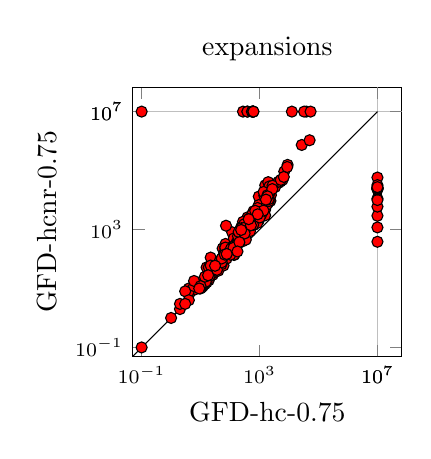
\begin{tikzpicture}
\begin{axis}[extra x tick style={grid=major}, extra x ticks=10000000, extra y tick style={grid=major}, extra y ticks=10000000, height=5cm, legend cell align=left, legend style={at={(1.3, 0.5)}}, title=expansions, width=5cm, xlabel=GFD-hc-0.75, xmin=0.05, xmode=log, ylabel=GFD-hcnr-0.75, ymin=0.05, ymode=log]
\addplot[color=red, mark=*, mark options={{draw=black}}, only marks] coordinates {
(226, 967) (6, 9) (981, 3311) (2144, 17941) (439, 1855) (942, 13116) (47, 66) (2121, 9781) (12, 12) (214, 686) (110, 283) (372, 890) (371, 930) (396, 958) (5143, 42522) (391, 2589) (58, 76) (11, 11) (125, 358) (169, 800) (43, 63) (275, 1834) (288, 1393) (937, 3229) (6046, 48299) (2695, 34370) (8954, 156081) (240, 1209) (95, 190) (19, 19) (1, 1) (173, 573) (4, 10) (1564, 31775) (106, 230) (175, 395) (46, 62) (14, 14) (70, 149) (37, 51) (2333, 9377) (296, 797) (22, 35) (27062, 739115) (123, 244) (38725, 10000000) (56, 228) (36, 41) (136, 290) (18, 25) (6890, 92912) (901, 2892) (227, 673) (137, 137) (1337, 6876) (607, 10000000) (622, 1783) (1458, 14012) (651, 2599) (103, 192) (16, 16) (275, 10000000) (1651, 7795) (32536, 10000000) (307, 954) (2437, 14770) (4389, 38253) (1805, 9221) (730, 2078) (10000000, 11219) (68, 248) (359, 929) (947, 2049) (27, 60) (70, 100) (891, 4609) (10000000, 2923) (48, 63) (26, 29) (10000000, 1180) (131, 318) (10000000, 57999) (40, 40) (164, 345) (118, 808) (2, 2) (34, 47) (24, 43) (3378, 27691) (639, 1422) (1469, 6939) (2176, 16918) (580, 10000000) (123, 212) (26, 33) (390, 10000000) (845, 1668) (302, 1070) (90, 150) (144, 407) (284, 1110) (306, 1402) (387, 10000000) (417, 1764) (13, 19) (73, 146) (92, 154) (391, 1046) (2036, 11460) (4401, 41680) (205, 694) (100, 202) (4, 6) (10, 10) (54, 95) (770, 3093) (604, 10000000) (53, 66) (552, 2794) (27, 38) (302, 699) (1971, 40492) (251, 850) (259, 1053) (941, 6750) (112, 314) (56, 73) (476, 878) (1538, 4638) (4, 8) (188, 381) (550, 10000000) (22, 112) (419, 1653) (245, 463) (142, 142) (6, 12) (602, 2919) (271, 760) (2155, 29010) (11, 17) (10000000, 24484) (1940, 7993) (101, 240) (60, 60) (499, 1732) (276, 542) (606, 10000000) (51, 66) (1741, 6855) (10000000, 5974) (10000000, 384) (474, 2375) (1548, 3031) (2754, 30702) (129, 385) (235, 1133) (737, 3522) (70, 324) (6, 18) (173, 421) (77, 104) (57, 114) (20, 26) (301, 1508) (13, 15) (607, 1430) (67, 139) (10000000, 10018) (623, 4157) (2, 3) (338, 1116) (16, 52) (1373, 18842) (134, 497) (260, 395) (0.100000, 10000000) (622, 10000000) (979, 3145) (133, 272) (5263, 48377) (12503, 10000000) (70, 160) (2060, 9235) (6652, 60966) (10000000, 25685) (103, 140) (80, 160) (10000000, 32097) (15, 17) (2025, 10591) (1165, 3337) (164, 351) (1844, 14576) (19, 52) (14, 25) (73, 1348) (170, 340) (10000000, 22877) (45, 89) (28, 55) (96, 236) (246, 1106) (164, 302) (335, 1194) (36, 43) (861, 5382) (3, 8) (119, 254) (342, 450) (2708, 23542) (8690, 132345) (1018, 2560) (53916, 10000000) (10, 12) (136, 233) (83, 195) (297, 735) (64, 163) (10000000, 24217) (442, 2329) (186, 594) (10000000, 26130) (1875, 13298) (0.100000, 0.100000) (49941, 1067776) (253, 755) (1652, 10340) (4, 4) (9, 10) (1362, 4383) (69, 244) (52, 77) (106, 219) (52, 104) (131, 240) (22, 60) (564, 3227) (3, 3) (10000000, 27397) (196, 828) (311, 735) (511, 1394) (31, 59) (207, 372) (238, 966) (715, 4320) (66, 141) (867, 3283) (429, 2248) (77, 148) (178, 180) (18, 28)
};
\addplot[color=black] coordinates {(0.050000, 0.050000) (10000000, 10000000)};
\end{axis}
\end{tikzpicture}
	\end{minipage}
	\hfill
	\begin{minipage}{0.2\textwidth}
		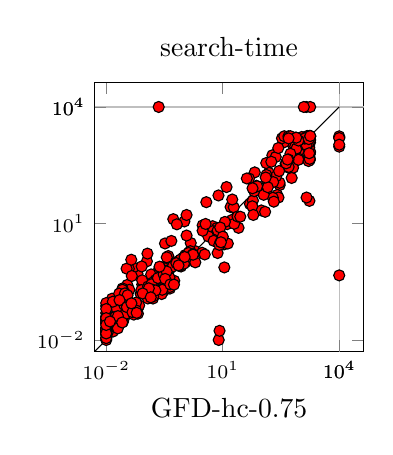
\begin{tikzpicture}
\begin{axis}[extra x tick style={grid=major}, extra x ticks=10000, extra y tick style={grid=major}, extra y ticks=10000, height=5cm, legend cell align=left, legend style={at={(1.3, 0.5)}}, title=search-time, width=5cm, xlabel=GFD-hc-0.75, xmin=0.005, xmode=log, ymin=0.005, ymode=log]
\addplot[color=red, mark=*, mark options={{draw=black}}, only marks] coordinates {
(0.028588, 0.035970) (0.698269, 1.030190) (0.034901, 0.262135) (98.691600, 21.673500) (0.012676, 0.017456) (1422.800045, 10000) (25.564400, 7.717710) (0.105115, 0.222073) (1.335820, 1.612330) (0.036071, 0.105629) (11.202300, 2.982330) (0.076990, 0.155101) (0.843372, 0.781518) (144.095000, 124.025000) (0.018737, 0.020747) (0.570090, 0.841492) (1733.526276, 605.803996) (0.066899, 0.069352) (0.063842, 0.506460) (1416.170875, 491.368920) (0.454279, 0.245628) (618.386006, 1200.902000) (1176.089915, 1605.396250) (118.259000, 61.971600) (0.152552, 0.316836) (0.962801, 1.322000) (1.118100, 1.017070) (0.244440, 0.749018) (0.010000, 0.032932) (0.010000, 0.016121) (0.039374, 0.195625) (388.243000, 1246.948000) (0.010000, 0.049424) (0.396773, 1.445910) (0.302142, 0.182898) (0.220770, 0.386856) (0.010000, 0.018436) (0.423347, 0.671825) (0.436588, 0.211109) (0.010000, 0.020001) (5.507420, 8.492880) (0.010000, 0.039269) (5.946540, 4.102760) (0.050820, 0.052995) (189.706000, 570.274000) (0.084698, 0.268282) (8.545920, 5.732110) (0.469501, 0.765802) (335.541000, 1564.624900) (0.450930, 0.818710) (7.133740, 7.685290) (0.318468, 0.704218) (50.208900, 31.798800) (0.326686, 3.059300) (416.354400, 345.446000) (5.594140, 6.334900) (1139.970000, 651.004000) (13.042300, 9.604810) (1746.234199, 432.524000) (0.049577, 0.738745) (59.958900, 38.902000) (1661.289171, 980.985170) (10000, 0.460674) (0.127264, 0.229988) (153.017000, 202.573000) (1714.700000, 457.336000) (757.336000, 1621.768800) (0.533816, 12.912700) (0.103409, 0.156985) (0.010000, 0.016005) (0.336299, 0.241045) (1.871030, 1.983460) (0.373961, 0.613401) (74.101300, 93.549400) (0.263021, 0.331453) (0.010000, 0.028483) (663.965000, 982.524200) (0.010000, 0.010000) (0.053153, 0.084408) (0.143701, 0.487279) (0.315772, 0.528561) (0.125928, 0.266322) (15.971500, 26.517700) (10000, 1627.377000) (0.904065, 1.232310) (1653.493405, 1492.140000) (10.286000, 3.358718) (1734.216734, 1796.834337) (0.030145, 0.057020) (475.666000, 278.382000) (0.084153, 0.343040) (7.384120, 1.734830) (0.010000, 0.074921) (66.795400, 206.862000) (0.232067, 0.677463) (1771.206562, 1776.525491) (293.137000, 97.591500) (0.017690, 0.029102) (0.159844, 0.116764) (131.815000, 359.863000) (1.029050, 11.276500) (1777.786578, 1731.373869) (1576.194000, 1674.393870) (0.065549, 0.047611) (0.010000, 0.013917) (0.010000, 0.036370) (1601.616220, 1300.257900) (1.081090, 1.534530) (0.018450, 0.065498) (3.038280, 8.932370) (0.027012, 0.029451) (1772.544357, 680.193979) (0.014849, 0.038325) (253.232000, 54.240800) (231.511000, 515.519147) (1658.562848, 870.148000) (131.346000, 64.949900) (0.035041, 0.067848) (0.014871, 0.016477) (0.475678, 3.550930) (10.809500, 2.896730) (10000, 1753.719500) (0.010866, 0.015410) (0.184775, 0.346383) (1685.361045, 1620.700000) (1.363950, 1.807730) (291.055000, 111.819000) (7.883260, 0.010000) (0.010000, 0.037374) (0.014167, 0.115752) (0.038213, 0.686321) (2.944550, 1.757220) (272.660000, 46.547300) (19.249400, 26.174800) (0.010000, 0.014208) (0.010000, 0.039580) (729.912000, 759.860000) (17.167000, 12.272200) (269.487506, 876.439600) (12.545600, 86.675500) (1.232960, 1.583710) (1081.618000, 1683.722300) (0.010000, 0.014132) (1766.634333, 1454.299136) (238.358000, 164.904000) (0.432221, 0.231120) (133.297000, 177.370000) (1663.683066, 1029.436750) (6.131140, 4.933490) (3.438020, 1.593020) (1758.205376, 1783.781586) (0.241276, 0.761414) (4.241070, 4.658860) (0.018404, 0.032512) (0.340572, 0.567627) (178.420000, 388.468952) (0.026297, 0.212369) (1724.742241, 645.736376) (0.070491, 0.077937) (0.267863, 0.152378) (804.670851, 1251.917400) (1762.888509, 721.047395) (0.010000, 0.017790) (0.033467, 0.687249) (0.163898, 0.307332) (1710.714415, 472.406000) (736.310000, 966.082000) (0.768340, 0.805476) (195.737000, 45.792900) (0.289497, 0.489038) (1.171650, 1.519770) (1.499469, 3.149330) (1764.762762, 1774.312790) (797.833000, 851.828000) (10000, 1583.554410) (0.617453, 0.880767) (0.080374, 0.192335) (8.277621, 0.017239) (0.564514, 0.334235) (1.661630, 1.133660) (0.019170, 0.039287) (0.025970, 0.196207) (0.051357, 0.045143) (648.176000, 272.150000) (0.021555, 0.156546) (1706.816900, 38.194500) (1687.463564, 904.648000) (0.742419, 1.086250) (1769.236499, 1218.177735) (1777.474492, 1380.888007) (0.017191, 0.039380) (10000, 951.470000) (113.268000, 54.767500) (0.361975, 1.344350) (0.819187, 1.177050) (948.512000, 455.875200) (0.045573, 0.444270) (0.010000, 0.020635) (1.463290, 1.934800) (0.058774, 0.091804) (497.959000, 285.837000) (0.010000, 0.089398) (1777.311833, 1747.171998) (19.678900, 9.818420) (0.161930, 0.133293) (0.120127, 0.239013) (0.058588, 0.057626) (891.031404, 436.559000) (0.117956, 0.117137) (1.174530, 4.896350) (1443.271400, 46.609200) (7.428120, 6.663120) (552.948000, 624.165201) (64.589600, 67.959200) (1660.644432, 882.358779) (1.323910, 1.743490) (1677.742200, 1722.741599) (0.030760, 0.046291) (0.146152, 0.271620) (1370.380000, 1027.360210) (0.258260, 0.432374) (0.010000, 0.026408) (1.425550, 1.400550) (1498.918146, 1791.039614) (1644.928015, 1190.920880) (0.010000, 0.030849) (0.342286, 0.258845) (1439.650000, 1050.638464) (0.028802, 0.081152) (0.019917, 0.019882) (3.781240, 35.365400) (1.969290, 0.996813) (283.281000, 224.346000) (0.010000, 0.018720) (0.010000, 0.014581) (0.010000, 0.037315) (1286.010000, 1541.540000) (0.014809, 0.096894) (1.722500, 1.619850) (0.111626, 1.059350) (1619.952000, 1749.966330) (0.214483, 0.394041) (0.277105, 0.196267) (1592.030000, 603.806000) (493.277000, 443.094000) (0.030347, 0.158542) (0.159614, 0.195324) (0.020044, 0.041174) (0.184487, 0.187838) (0.301257, 0.488516) (206.741000, 36.417300) (0.010000, 0.011416) (3.036980, 6.504920) (596.206000, 148.614000) (199.589000, 116.222000) (0.010000, 0.062724) (1789.482011, 10000) (1707.853347, 515.476248) (13.526000, 3.043170) (0.035383, 0.142023) (0.224661, 10000) (0.034147, 0.075056) (77.161700, 90.582500) (1.720740, 1.572360) (47.429400, 143.774000) (0.021989, 0.106302) (1623.614532, 405.088000) (383.890000, 1762.908200) (0.034113, 0.070111) (0.125204, 0.214028) (0.518536, 0.779330) (0.640766, 0.952026) (1227.620049, 10000) (431.008200, 353.447000) (0.047489, 0.051975) (144.822000, 85.855617) (123.469000, 19.974600) (1.172390, 16.541900) (467.231000, 442.250000) (0.010000, 0.011177) (0.010000, 0.014748) (57.722400, 27.684000) (11.375700, 10.975200) (3.619580, 9.717080) (0.425383, 0.404327) (41.795800, 144.178000) (8.615770, 7.887453) (1.001990, 0.921792) (7.770440, 52.692900) (1303.219013, 1556.323630) (0.360615, 0.580445) (5.839410, 3.578390) (17.591600, 41.409400) (0.010000, 0.036523) (0.328808, 0.374332) (1730.882848, 460.795000) (0.236435, 0.771949) (8.162680, 2.819640) (11.014700, 0.738677) (0.060770, 0.049957) (1.047520, 1.369580) (8.794420, 3.365036) (888.817047, 1367.304900) (0.082029, 0.782949) (0.086820, 0.157739) (128.033000, 152.502000) (0.658473, 9.510060) (1681.779983, 643.561000) (0.010000, 0.024396) (0.115375, 1.675830) (0.044538, 0.087778) (492.439000, 1759.505530) (24.114600, 15.114100) (552.977460, 1768.530000) (0.025835, 0.028197) (10.037100, 4.579630) (58.608700, 80.624300) (0.446390, 0.269813) (1646.521945, 1487.977000) (780.534925, 1620.694779) (0.012502, 0.029946) (10000, 1068.097000) (61.306800, 16.581000) (0.044197, 1.165820) (1795.541050, 1785.137790) (28.354100, 14.943300) (8.982500, 3.279597) (0.727492, 0.834750) (0.554831, 0.266699) (0.140079, 0.125292) (497.025000, 1552.814030)
};
\addplot[color=black] coordinates {(0.0050000, 0.0050000) (10000, 10000)};
\end{axis}
\end{tikzpicture}
	\end{minipage}

	\caption{Comparison of expansions and search time per task of $h^{C}$ with and 
	without the reuse of the heuristic for oversubscription IPC domains}
\end{figure}

\FloatBarrier
\subsubsection{Top Down vs. Bottom Up}
%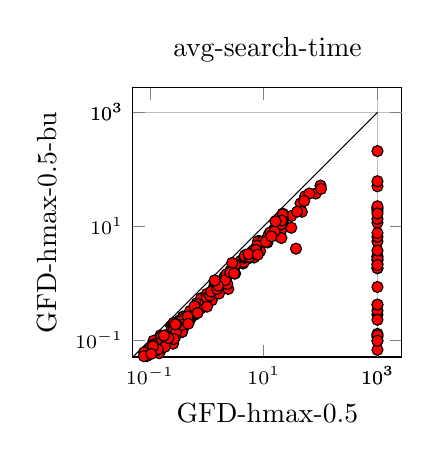
\begin{tikzpicture}
\begin{axis}[extra x tick style={grid=major}, extra x ticks=1000, extra y tick style={grid=major}, extra y ticks=1000, height=5cm, legend cell align=left, legend style={at={(1.3, 0.5)}}, title=avg-search-time, width=5cm, xlabel=GFD-hmax-0.5, xmin=0.05, xmode=log, ylabel=GFD-hmax-0.5-bu, ymin=0.05, ymode=log]
\addplot[color=red, mark=*, mark options={{draw=black}}, only marks] coordinates {
(0.001429, 0.002000) (0.071133, 0.040180) (0.001695, 0.001429) (0.050646, 0.034464) (0.010962, 0.006387) (0.008600, 0.006411) (0.009221, 0.006207) (1000, 50.163333) (8.360400, 5.476938) (0.452991, 0.259884) (0.001105, 0.000897) (0.001825, 0.001325) (0.119589, 0.033672) (0.010318, 0.007335) (0.873832, 0.496353) (0.005781, 0.003713) (5.337129, 2.904212) (82.387333, 37.442200) (0.001159, 0.001000) (1000, 0.006686) (0.000624, 0.000483) (1000, 0.027209) (0.030600, 0.018362) (44.555357, 25.113208) (0.069041, 0.038820) (0.266086, 0.103948) (0.009002, 0.005851) (0.526185, 0.247239) (21.689600, 16.134700) (1000, 0.001462) (0.063196, 0.034049) (0.011538, 0.006400) (1000, 1.817921) (0.000385, 0.000227) (1000, 208.502857) (1000, 0.003827) (1.163240, 0.505172) (0.188711, 0.103096) (0.250886, 0.114913) (0.159044, 0.116881) (0.003087, 0.002500) (0.115150, 0.062686) (0.005632, 0.001511) (0.169788, 0.099449) (0.236566, 0.175962) (8.688683, 3.655433) (0.248990, 0.158929) (0.003333, 0.002500) (0.000461, 0.000460) (0.000350, 0.000329) (0.001429, 0.000625) (0.001876, 0.001286) (0.000286, 0.000201) (0.125803, 0.084012) (0.002738, 0.001422) (0.042130, 0.021030) (0.001250, 0.000667) (0.613453, 0.276530) (2.388558, 0.786778) (0.000388, 0.000266) (0.001429, 0.000345) (0.007991, 0.004587) (30.637818, 9.373455) (0.010000, 0.005600) (0.010936, 0.007522) (0.003480, 0.003333) (4.326176, 2.200241) (0.364409, 0.226615) (0.097490, 0.068047) (0.000272, 0.000191) (0.012348, 0.006155) (0.004990, 0.003136) (1000, 0.278895) (6.374113, 3.395080) (0.022412, 0.014778) (0.071796, 0.039842) (1.438643, 0.947096) (0.001580, 0.001195) (0.247814, 0.115492) (30.581143, 15.099200) (0.031221, 0.023927) (0.050738, 0.030858) (2.048733, 1.278755) (22.157533, 13.006667) (0.000667, 0.002000) (0.188766, 0.103459) (0.665380, 0.440857) (0.001766, 0.001456) (0.000394, 0.000264) (1.329933, 0.839270) (21.655800, 16.595619) (0.023436, 0.013074) (0.019523, 0.010253) (0.001239, 0.001044) (0.803260, 0.539691) (0.073259, 0.043719) (0.040470, 0.032415) (15.477600, 7.076660) (1000, 2.958017) (1000, 0.009241) (1000, 0.014676) (0.018188, 0.013655) (0.228521, 0.119114) (0.000588, 0.000313) (0.000240, 0.000167) (0.000252, 0.000176) (1000, 20.962500) (7.222350, 3.954912) (0.469708, 0.270066) (16.610300, 6.847300) (1000, 2.877075) (0.000667, 0.000833) (0.003005, 0.002156) (0.021625, 0.011734) (3.150679, 1.466884) (0.793073, 0.538514) (0.003123, 0.002500) (0.084103, 0.039979) (0.045318, 0.021105) (1000, 2.173240) (0.057204, 0.028428) (0.000422, 0.000291) (1.442386, 0.846733) (0.001410, 0.000730) (0.044860, 0.029532) (0.015366, 0.011191) (1000, 5.369070) (1.002741, 0.477862) (0.019307, 0.009968) (0.000222, 0.000157) (1000, 0.326723) (0.003156, 0.002550) (3.029860, 1.867422) (2.608897, 1.666620) (0.381139, 0.256964) (0.000611, 0.000446) (5.069123, 2.638405) (0.000667, 0.000769) (0.022530, 0.012914) (1.463300, 0.826738) (1.385552, 0.743483) (1.534127, 0.816008) (0.289903, 0.138536) (8.040467, 5.429147) (0.058378, 0.039798) (53.486154, 33.480520) (0.065932, 0.024787) (1000, 0.033399) (0.151287, 0.067430) (1000, 0.003321) (0.200057, 0.103517) (0.000424, 0.000275) (1000, 20.041429) (7.976392, 5.374367) (0.000272, 0.000196) (1.118741, 0.520131) (0.024038, 0.014155) (0.387724, 0.162053) (1000, 0.096460) (11.532417, 5.468295) (4.004103, 2.474353) (0.710668, 0.425508) (4.470700, 2.325833) (0.156205, 0.073450) (1.002747, 0.591638) (0.009013, 0.006248) (0.004384, 0.002682) (0.012317, 0.006351) (1000, 0.127871) (0.108699, 0.059146) (0.000323, 0.000263) (0.037165, 0.019675) (0.000471, 0.000296) (99.785000, 51.635077) (4.875143, 3.144186) (0.129165, 0.087883) (0.000748, 0.000909) (6.322040, 3.589856) (9.553600, 5.352322) (1000, 0.113104) (1000, 0.003040) (0.000396, 0.000277) (0.002500, 0.001250) (1000, 6.504100) (0.011930, 0.007912) (0.154480, 0.068231) (0.003197, 0.002459) (1000, 0.006698) (0.008798, 0.005182) (0.386242, 0.254011) (0.115772, 0.096543) (0.003542, 0.001858) (0.000851, 0.000909) (7.622333, 4.530745) (0.000726, 0.000909) (12.770700, 6.692900) (0.509123, 0.295418) (0.000667, 0.000714) (2.227850, 0.978805) (1.033320, 0.563050) (4.618160, 2.788164) (1.385687, 0.980771) (0.006634, 0.003904) (0.331334, 0.221594) (0.113277, 0.081868) (0.000495, 0.001111) (0.129887, 0.062558) (0.047159, 0.026693) (0.000667, 0.001667) (0.003246, 0.001609) (0.016132, 0.007849) (0.010830, 0.006783) (0.000824, 0.001429) (1.151620, 0.572065) (0.003290, 0.002486) (0.045508, 0.020755) (0.001163, 0.000969) (0.010743, 0.005319) (0.000335, 0.000233) (0.457089, 0.248968) (0.097398, 0.067741) (0.001362, 0.001118) (0.206093, 0.124716) (0.000667, 0.000909) (0.122337, 0.068965) (1000, 0.416645) (0.004154, 0.002754) (0.003630, 0.002630) (0.042672, 1000) (0.000855, 0.000567) (0.008628, 0.005923) (0.491631, 0.217085) (1.542982, 0.805962) (0.005224, 0.003701) (1000, 18.378082) (0.143032, 0.067281) (0.044971, 0.028678) (0.011652, 0.006005) (0.012568, 0.010338) (1000, 0.033609) (0.012353, 0.006626) (0.003519, 0.001449) (12.656800, 7.530291) (4.651886, 2.999771) (0.262860, 0.196600) (1000, 0.011360) (15.118200, 8.608114) (0.002741, 0.001977) (0.000417, 0.000357) (0.000556, 0.000174) (0.009194, 0.006152) (0.003021, 0.002278) (0.562133, 0.305426) (0.113487, 0.065930) (1.541543, 0.867563) (0.778484, 0.357428) (0.001266, 0.001006) (0.085862, 0.031413) (0.255929, 0.085909) (0.000327, 0.000242) (46.849733, 17.890940) (1000, 0.003021) (0.041437, 0.030166) (0.000323, 0.001667) (0.409164, 0.200858) (0.321927, 0.143480) (1000, 11.511667) (0.003333, 0.003333) (0.043052, 0.018455) (0.010686, 0.006294) (0.260222, 0.167632) (1.000307, 0.602146) (0.001159, 0.000970) (0.000769, 0.001667) (0.021405, 0.012779) (0.000538, 0.000392) (21.607867, 16.099900) (1.086754, 0.624950) (0.003246, 0.002398) (0.026093, 0.020611) (4.649643, 2.979029) (0.638418, 0.306493) (19.161800, 10.041880) (0.000867, 0.000909) (1000, 0.025739) (2.739316, 1.645610) (1000, 2.505937) (0.015366, 0.007176) (0.260313, 0.197431) (20.105333, 8.249657) (38.740867, 17.924180) (0.002542, 0.001487) (0.001266, 0.001010) (1000, 61.626818) (0.000462, 0.000385) (0.005160, 0.003457) (0.000904, 0.000659) (1.465235, 0.957527) (0.030449, 0.020872) (0.002497, 0.001858) (1000, 0.007324) (0.367451, 0.137932) (0.129373, 0.062189) (0.087538, 0.043367) (0.058911, 0.029825) (0.371337, 0.233421) (1000, 0.120055) (0.001162, 0.000965) (0.010000, 0.005000) (4.651729, 2.997200) (2.051150, 1.271885) (0.033813, 0.022287) (0.507384, 0.321426) (11.640067, 5.159912) (0.000432, 0.000296) (13.813467, 7.378800) (1000, 1.837496) (0.245544, 0.158658) (0.001595, 0.001120) (2.300840, 0.963820) (0.338447, 0.194598) (0.003299, 0.001943) (0.636649, 0.295137) (16.623654, 9.995557) (0.000278, 0.000197) (0.146110, 0.058390) (0.963298, 0.459176) (0.000462, 0.000625) (0.087272, 0.049423) (0.012697, 0.008152) (0.001429, 0.002500) (0.111013, 0.047400) (20.520182, 6.191520) (2.221180, 1.318075) (0.005272, 0.000959) (0.049628, 0.029552) (0.018094, 0.014121) (0.464614, 0.222760) (37.012000, 4.019033) (0.061385, 0.029121) (0.025510, 0.011129) (0.000790, 0.000544) (0.002318, 0.001735) (0.009093, 0.006237) (0.345024, 0.211273) (0.010460, 0.006331) (0.340256, 0.171275) (0.000965, 0.000745) (5.636220, 2.785188) (1000, 0.007318) (0.002000, 0.002000) (0.003293, 0.002230) (0.000427, 0.000332) (0.022221, 0.015490) (0.079103, 0.060453) (1000, 0.851902) (0.001429, 0.001250) (0.000343, 0.000244) (0.003112, 0.002457) (0.029510, 0.017389) (1.166615, 0.511979) (0.013046, 0.007884) (0.008417, 0.006599) (0.002820, 0.001992) (0.000233, 0.000217) (0.072970, 0.043861) (2.316147, 1.379980) (0.000714, 0.000333) (0.001487, 0.001157) (1000, 0.043166) (3.161393, 2.104042) (1000, 22.353118) (1.005070, 0.643737) (0.002957, 0.002071) (0.000526, 0.000323) (0.035531, 0.023916) (1000, 0.001468) (0.028354, 0.022213) (0.000885, 0.000909) (0.067105, 0.034954) (0.000214, 0.000177) (21.187091, 11.822422) (0.037808, 0.024018) (0.044825, 0.025311) (0.085910, 0.032284) (0.263155, 0.168433) (0.000310, 0.000232) (1000, 0.011343) (1.132087, 0.587428) (0.111824, 0.046294) (0.032990, 0.019460) (1000, 7.577621) (2.215160, 1.428830) (0.953538, 0.454688) (0.000203, 0.000157) (0.002642, 0.002008) (0.001429, 0.001429) (0.461908, 0.258074) (0.002381, 0.001757) (1.617768, 0.701199) (0.171198, 0.092887) (63.711267, 37.541000) (0.040989, 0.028568) (1.224010, 0.496975) (0.009563, 0.005460) (0.023291, 0.014982) (0.125339, 0.079845) (12.059250, 6.774609) (0.000319, 0.001429) (0.003661, 0.002600) (0.037381, 0.020087) (0.005222, 0.003491) (0.000359, 0.000248) (0.271009, 0.115676) (1.005740, 0.548222) (0.001233, 0.000933) (6.773367, 2.811917) (1000, 0.003831) (0.000286, 0.000188) (0.210873, 0.101863) (0.118651, 0.069606) (21.439818, 11.677911) (0.002586, 0.001858) (0.000381, 0.001250) (0.365489, 0.138145) (0.011829, 0.006660) (0.000298, 0.000205) (0.153714, 0.120360) (0.000387, 0.000257) (0.010000, 0.006958) (0.000433, 0.000325) (0.001407, 0.001429) (0.003217, 0.002000) (0.120725, 0.032567) (13.187714, 7.782609) (0.000338, 0.000269) (0.000769, 0.000313) (1000, 2.629097) (0.028732, 0.016032) (10.925400, 5.311175) (0.000385, 0.000228) (0.000403, 0.000295) (1000, 0.014484) (0.014160, 0.010347) (0.263516, 0.151421) (0.004720, 0.003446) (0.001936, 0.001294) (1000, 3.731000) (0.000353, 0.000305) (1.138746, 0.603688) (0.280666, 0.115284) (1000, 0.003004) (2.119567, 1.123594) (0.012772, 0.008150) (0.003522, 0.002245) (0.021783, 0.014221) (0.605173, 0.390790) (0.083691, 0.035309) (0.289676, 0.140144) (6.648408, 3.778625) (0.027928, 0.013907) (0.015858, 0.007458) (0.156739, 0.071959) (2.802910, 2.248239) (2.809381, 2.244979) (0.001111, 0.001111) (0.006747, 0.004432) (5.649768, 2.890857) (20.361867, 10.746913) (7.294142, 3.824038) (0.115819, 0.071450) (0.000400, 0.000145) (0.002427, 0.001517) (0.057322, 0.034047) (0.022306, 0.015374) (0.077980, 0.044825) (0.014975, 0.009243) (20.743962, 12.545864) (0.001569, 0.001016) (51.709600, 27.740400) (0.014442, 0.010330) (1000, 0.066901) (1.009426, 0.384670) (0.008022, 0.005047) (0.012840, 0.007204) (1000, 0.416290) (1.636298, 0.652251) (0.060683, 0.024307) (0.047749, 0.025824) (0.005538, 0.001871) (0.363597, 0.183062) (5.424400, 3.223775) (0.000320, 0.000263) (0.012415, 0.007333) (0.001111, 0.000333) (0.132032, 0.065524) (0.000374, 0.000268) (0.292780, 0.190163) (1.461121, 0.838731) (0.190797, 0.107713) (0.044311, 0.027196) (0.009253, 0.006274) (0.027435, 0.014447) (0.158187, 0.113830) (0.133457, 0.085645) (1.198453, 0.707420) (1000, 13.418107) (0.003954, 0.002565) (0.691402, 0.298273) (0.281333, 0.187904) (1.514883, 0.784406) (102.216000, 45.260800) (0.000247, 0.000173) (0.001269, 0.001429) (1000, 0.002259) (0.087434, 0.051780) (0.000304, 0.000277) (0.057383, 0.028109) (1000, 0.096602) (0.004608, 0.003258) (0.000724, 0.000909) (16.214357, 12.191643) (15.522233, 8.161300) (0.077904, 0.035470) (0.263773, 0.103897) (0.000366, 0.000320) (2.591759, 1.536633) (1000, 0.225613) (0.000778, 0.000909) (0.003907, 0.003333) (1000, 2.076491) (0.010000, 0.005210) (1000, 0.007195) (0.000411, 0.000283) (0.009198, 0.006493) (0.006166, 0.004045) (0.078412, 0.051788) (0.000316, 0.000221) (0.247406, 0.016828) (0.001128, 0.001041) (3.021714, 1.475613) (0.000685, 0.000523) (0.003575, 0.002796) (0.055595, 0.029394) (1000, 16.704239) (0.000264, 0.000199) (16.130214, 12.108071) (13.681533, 6.618000) (0.000207, 0.000156) (0.063890, 0.035979) (0.021760, 0.017048) (0.183268, 0.075573) (0.473550, 0.192443) (0.211084, 0.107855) (0.137698, 0.068407) (0.114234, 0.082227) (0.113718, 0.077052) (0.001565, 0.001166) (7.879200, 3.152514) (0.000829, 0.001667) (0.000317, 0.000213) (1.582643, 0.895920) (1.375920, 1.111581) (1.382980, 1.110912) (0.001212, 0.000702) (0.004598, 0.003340) (0.008746, 0.006358) (0.017132, 0.010615) (0.105230, 0.056814) (1000, 0.043771) (0.176722, 0.119142)
};
\addplot[color=black] coordinates {(0.050000, 0.050000) (1000, 1000)};
\end{axis}
\end{tikzpicture}


\begin{figure}[ht]
	\small
\begin{tabular}{l||rr||rr|rr||rr}
	& \multicolumn{2}{c}{0.25} & \multicolumn{4}{c}{0.5} & \multicolumn{2}{c}{0.75} \\\hline
		& tp c & bu & tp c & bu c & td fn & bu fn & td c & bu c \\\hline
		airport (28) & 24 & 25 & 19 & 21 & 0.71 & 0.67 & 19 & 21\\
		barman (4) & 4 & 4 & 4 & 4 & 0.88 & 0.88 & 4 & 4\\
		blocks (28) & 27 & 28 & 21 & 23 & 0.93 & 0.39 & 17 & 18\\
		data-network (12) & 12 & 12 & 12 & 12 & 0.65 & 0.60 & 12 & 12\\
		depot (7) & 7 & 7 & 7 & 7 & 0.91 & 0.52 & 4 & 4\\
		driverlog (13) & 13 & 13 & 10 & 11 & 0.86 & 0.58 & 8 & 9\\
		elevators (40) & 40 & 40 & 40 & 40 & 0.89 & 0.65 & 33 & 35\\
		floortile (13) & 6 & 7 & 2 & 2 & 0.80 & 0.67 & 2 & 2\\
		freecell (15) & 15 & 15 & 15 & 15 & 0.94 & 0.60 & 14 & 14\\
		ged (15) & 10 & 15 & 10 & 12 & 0.80 & 0.47 & 10 & 10\\
		grid (2) & 2 & 2 & 2 & 2 & 0.69 & 0.56 & 2 & 2\\
		gripper (7) & 5 & 7 & 4 & 5 & 0.88 & 0.65 & 5 & 4\\
		hiking (9) & 9 & 9 & 9 & 9 & 0.61 & 0.61 & 9 & 9\\
		logistics (26) & 22 & 25 & 15 & 18 & 0.84 & 0.68 & 12 & 12\\
		miconic (141) & 56 & 69 & 45 & 50 & 0.82 & 0.67 & 45 & 45\\
		mprime (22) & 22 & 22 & 22 & 22 & 0.59 & 0.59 & 22 & 22\\
		mystery (17) & 17 & 17 & 17 & 17 & 0.63 & 0.62 & 15 & 16\\
		nomystery (14) & 14 & 14 & 10 & 10 & 0.92 & 0.63 & 8 & 8\\
		openstacks (47) & 24 & 47 & 22 & 47 & 0.99 & 0.07 & 20 & 43\\
		parking (5) & 0 & 5 & 0 & 0 & - & - & 0 & 0\\
		pathways-noneg (5) & 5 & 5 & 4 & 4 & 0.77 & 0.64 & 4 & 4\\
		pipesworld-nt (17) & 17 & 17 & 16 & 17 & 0.84 & 0.69 & 16 & 16\\
		psr-small (49) & 48 & 48 & 48 & 47 & 0.55 & 0.86 & 47 & 46\\
		rovers (8) & 8 & 8 & 7 & 7 & 0.84 & 0.74 & 6 & 6\\
		satellite (7) & 7 & 7 & 6 & 6 & 0.94 & 0.49 & 4 & 5\\
		scanalyzer (27) & 9 & 9 & 9 & 9 & 0.86 & 0.53 & 9 & 9\\
		snake (7) & 1 & 3 & 1 & 2 & 0.91 & 0.24 & 1 & 1\\
		sokoban (50) & 49 & 50 & 47 & 48 & 0.73 & 0.80 & 42 & 43\\
		storage (15) & 15 & 15 & 15 & 15 & 0.75 & 0.75 & 15 & 15\\
		tetris (6) & 2 & 5 & 2 & 2 & 0.80 & 0.82 & 3 & 2\\
		tidybot (23) & 23 & 23 & 23 & 23 & 0.92 & 0.43 & 7 & 15\\
		tpp (7) & 7 & 7 & 6 & 7 & 0.83 & 0.59 & 6 & 6\\
		transport (23) & 23 & 23 & 23 & 23 & 0.88 & 0.59 & 23 & 23\\
		trucks (10) & 10 & 10 & 6 & 7 & 0.89 & 0.70 & 6 & 6\\
		zenotravel (13) & 12 & 13 & 8 & 9 & 0.89 & 0.66 & 8 & 8\\\hline
		Sum & 565 & 626 & 507 & 553 &  &  & 458 & 495\\
	\end{tabular}
	\caption{Comparison of coverage per cost bound for top-down vs bottom-up meta search.
	For cost-bound=0.5 there is (\#meta search nodes/maximinal number of meta search nodes) displayed.Planner $A^*$ with $h^{max}$}
	\rebecca{These are only preliminary results. There are still some domains missing because of a bug in 
		the bottom-up version. The missing domains are in favor of the top-down version.
		But the overall result should stay the same. Bottom-up often has to solve less nodes which can
	improve the coverage. Strongest difference in openstacks.}
\end{figure}


\begin{figure}[ht]
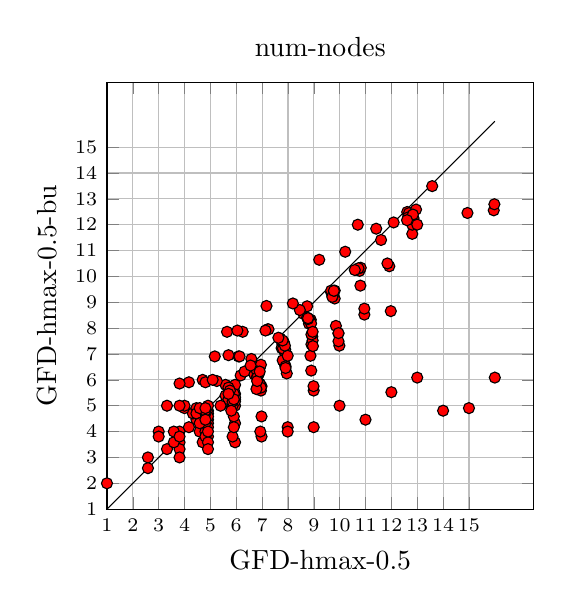
\begin{tikzpicture}
\begin{axis}[extra x tick style={grid=major},
	extra x ticks=100000,
grid,
extra y tick style={grid=major},
extra y ticks=100000,
height=7cm,
legend cell align=left,
legend style={at={(1.3,0.5)}},
title=num-nodes,
width=7cm,
xlabel=GFD-hmax-0.5,
xmin=1,
xmode=log,
ylabel=GFD-hmax-0.5-bu,
ymin=1,
ymode=log,
log basis x =2, log basis y=2, grid,
xtick={1,2,4,8,16,32,64,128,256,512,1024, 2048, 4096,8192,16384},	
xticklabels={1,2,3,4,5,6,7,8,9,10,11,12,13,14,15},
ytick={1,2,4,8,16,32,64,128,256,512,1024, 2048, 4096,8192,16384},	
yticklabels={1,2,3,4,5,6,7,8,9,10,11,12,13,14,15},
]
\addplot[color=red, mark=*, mark options={{draw=black}}, only marks] coordinates {
(31, 6) (992, 184) (194, 188) (31, 19) (225, 144) (12, 12) (56, 26) (56, 25) (3132, 2882) (832, 2048) (872, 594) (25, 116) (38, 116) (13, 32) (11, 11) (60, 44) (5, 5) (236, 160) (60, 29) (7, 6) (255, 9) (16383, 15) (62, 24) (15, 11) (31, 22) (510, 16) (29, 7) (214, 230) (120, 64) (8, 15) (29, 17) (448, 283) (3284, 2796) (10, 13) (6114, 5760) (7, 5) (408, 333) (52, 37) (25, 21) (15, 14) (48, 56) (13, 10) (111, 79) (1364, 1840) (594, 992) (30, 21) (63, 27) (36, 36) (118, 48) (124, 38) (28, 15) (9, 30) (11, 15) (240, 83) (7, 8) (495, 111) (12, 8) (15, 13) (63, 7) (437, 347) (31, 16) (9, 9) (24, 21) (176, 208) (246, 102) (115, 87) (14, 9) (1023, 11) (61, 28) (31, 18) (3201, 2487) (104, 97) (24, 28) (214, 170) (117, 68) (3968, 3076) (228, 160) (112, 90) (57, 42) (1552, 1360) (296, 800) (8191, 14) (992, 216) (15, 10) (63, 12) (116, 73) (15, 7) (58, 38) (238, 145) (29, 16) (13, 6) (55, 45) (900, 646) (27, 19) (127, 9) (15, 16) (14, 8) (7, 4) (14, 12) (110, 84) (108, 75) (15, 9) (31, 20) (26, 19) (74, 124) (3708, 2437) (4, 8) (30, 23) (62, 48) (111, 54) (219, 163) (26, 25) (15, 12) (13, 12) (62, 26) (407, 350) (34, 60) (6, 6) (8, 16) (14, 30) (119, 72) (56, 35) (29, 22) (120, 46) (26, 62) (255, 24) (429, 308) (28, 24) (30, 24) (11, 13) (31, 28) (33, 120) (14, 10) (112, 74) (61, 8) (420, 296) (118, 80) (59, 38) (508, 80) (35, 60) (448, 350) (76, 124) (31, 10) (55, 25) (56, 40) (19, 31) (31828, 3010) (6, 8) (5, 16) (146, 248) (248, 92) (14, 7) (15, 6) (40, 40) (2047, 23) (239, 41) (15, 8) (15731, 2805) (3, 4) (2016, 202) (254, 27) (30, 12) (4, 7) (3648, 2688) (127, 8) (32372, 3544) (7, 7) (14, 13) (30, 22) (111, 92) (219, 167) (127, 61) (7, 16) (56, 34) (21, 16) (438, 348) (15, 5) (72, 232) (240, 108) (1, 2) (7, 29) (29, 18) (3, 3) (892, 400) (848, 638) (30, 9) (26, 26) (2176, 2176) (18, 60) (14, 14) (12, 10) (234, 61) (248, 116) (3584, 1602) (56, 31) (47, 47) (250, 79) (30, 19) (3584, 2048) (27, 24) (32767, 34) (17, 32) (60, 40) (463, 136) (28, 14) (70, 120) (14, 11) (1938, 672) (12, 15) (768, 608) (99, 99) (1841, 725) (26, 22) (4095, 2052) (3113, 2312) (496, 90) (4095, 34) (120, 44) (14, 15) (496, 112)
};
\addplot[color=black] coordinates {(0.050000, 0.050000) (32767, 32767)};
\end{axis}
\end{tikzpicture}

\caption{Comparison of the number of nodes in the meta search tree for the top-down and bottom-up meta search.
	Planner $A^*$ with $h^{max}$}
\end{figure}


\FloatBarrier
\newpage
\subsubsection*{Action Set Properties}

\begin{figure}[ht]
	\begin{tabular}{l|r|rrrrrrrrrr}
		& & \multicolumn{10}{c}{\# properties} \\
		domain & \#goals & 1 & 2 & 3 & 4 & 5 & 6 & 7 & 8 & 9 & 10 \\\hline
		nomystery & 2 & 10 & 10 & 10 & 10 & 10 & 10 & 10 & 10 & 10 & 10\\\hline
				& 3 & 10 & 10 & 10 & 10 & 10 & 10 & 10 & 10 & 10 & 10\\\hline
				& 4 & 10 & 10 & 10 & 10 & 9 & 9 & 9 & 9 & 8 & 7\\\hline
				& 5 & 10 & 10 & 10 & 10 & 10 & 8 & 4 & 2 & 2 & 2\\\hline
				& 6 & 10 & 9 & 8 & 8 & 7 & 2 & 0 & 2 & 2 & 2\\\hline\hline
		openstacks & 1 & 10 & 10 & 10 & 10 & 10 & 10 & 10 & 10 & 10 & - \\\hline
				& 1 & 10 & 10 & 10 & 10 & 10 & 10 & 10 & 10 & 10 & - \\\hline
				& 2 & 10 & 10 & 10 & 10 & 10 & 10 & 10 & 10 & 10 & - \\\hline
				& 3 & 10 & 10 & 10 & 10 & 10 & 10 & 10 & 10 & 10 & - \\\hline
				& 4 & 10 & 10 & 10 & 10 & 10 & 10 & 10 & 10 & 10 & - \\\hline
				& 5 & 10 & 10 & 10 & 10 & 10 & 10 & 10 & 10 & 10 & - \\\hline
				& 6 & 10 & 10 & 10 & 10 & 10 & 10 & 10 & 10 & 10 & - \\\hline
				& 7 & 10 & 10 & 10 & 10 & 10 & 10 & 10 & 10 & 10 & - \\\hline
				& 8 & 10 & 10 & 10 & 10 & 10 & 10 & 10 & 10 & 10 & - \\\hline
				& 9 & 10 & 10 & 10 & 10 & 10 & 10 & 10 & 10 & 10 & - \\\hline\hline
		rovers & 2 & 10 & 10 & 10 & 10 & 10 & 8 & 5 & 2 & 2 &- \\\hline
				& 4 & 9 & 6 § & 6 & 2 & 0 & 0 & 0 & 0 & 0 & - \\\hline
				& 6 & 1 & 0 & 0 & 0 & 0 & 0 & 0 & 0 & 0 & - \\\hline 
				& 8 & 1 & 0 & 0 & 0 & 0 & 0 & 0 & 0 & 0 & - \\\hline 
				& 10 & 1 & 0 & 0 & 0 & 0 & 0 & 0 & 0 & 0 & - \\\hline 
				& 12 & 1 & 0 & 0 & 0 & 0 & 0 & 0 & 0 & 0 & - \\\hline 
				& 14 & 1 & 0 & 0 & 0 & 0 & 0 & 0 & 0 & 0 & - \\\hline 
				& 16 & 1 & 0 & 0 & 0 & 0 & 0 & 0 & 0 & 0 & - \\\hline 
				& 18 & 1 & 0 & 0 & 0 & 0 & 0 & 0 & 0 & 0 & - \\\hline\hline
		TPP & 3 & 10 & 10 & 10 & 10 & 10 & 10 & 10 & 10 & 10 & 10\\\hline
			& 4 & 10 & 10 & 10 & 10 & 10 & 10 & 10 & 10 & 10 & 10\\\hline
			& 5 & 10 & 10 & 10 & 10 & 10 & 10 & 10 & 10 & 8 & 3\\\hline
			& 6 & 10 & 10 & 10 & 10 & 10 & 8 & 3 & 1 & 1 & 1\\\hline


	\end{tabular}
	\caption{Coverage for $h^{max}$ and top-down meta-search, 10 instances per \# goals and \# properties combination.
	For nomystery and TPP is the size of the locations fixed to 6 locations respectively 5 markets and the fuel is the 
	minimal amount needed to solve the task.
	The original goal facts are hard goals and the property-goal-facts are soft-goals.}
\end{figure}

\rebecca{
	At least in nomystery it seams to be difficult to generated action set properties that can be satisfied if we use 
	a constraint of 1 for the fuel. Therefore in most cases the MUGS are simply all goal-facts + one property.
}


%\begin{figure}[ht]
\centering
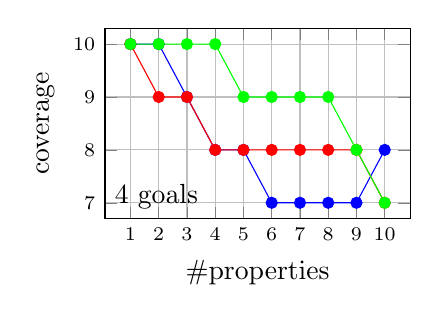
\begin{tikzpicture}
	\begin{axis}[
		title={4 goals},
		every axis title/.style={above right,at={(0,0)}},
		height=4cm,
		width=0.45\textwidth,
		xlabel=\#properties,
		ylabel=coverage,
		ytick={1,2,3,4,5,6,7,8,9,10},
		xtick={1,2,3,4,5,6,7,8,9,10},
		%xmin=0,
		%xmax=10,
		%ymin=0,
		%ymax=10,
		grid,
		%ybar,
		%bar width=2pt,
		legend style={at={(0.5,1.15)}, anchor=north,legend columns=-1},
		%mark options={%
		%	scale=2,fill=yellow!80!black,draw=black
		%}
	]
	\addplot+[blue,mark=*, mark options={fill=blue}] coordinates {
				(1,10) (2,10) (3,9) (4,8) (5,8) (6,7) (7,7) (8,7) (9,7) (10,8)
	};
	\addplot+[red,mark=*, mark options={fill=red}] coordinates {
				(1,10) (2,9) (3,9) (4,8) (5,8) (6,8) (7,8) (8,8) (9,8) (10,7)
	};
	\addplot+[green,mark=*, mark options={fill=green}] coordinates {
				(1,10) (2,10) (3,10) (4,10) (5,9) (6,9) (7,9) (8,9) (9,8) (10,7)
	};

	
	%\legend{hC, hC no reuse, hmax}
	\end{axis}
\end{tikzpicture}
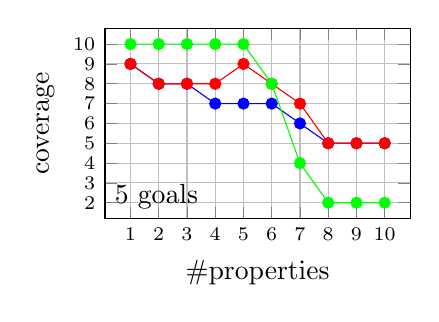
\begin{tikzpicture}
	\begin{axis}[
		title={5 goals},
		every axis title/.style={above right,at={(0,0)}},
		height=4cm,
		width=0.45\textwidth,
		xlabel=\#properties,
		ylabel=coverage,
		ytick={1,2,3,4,5,6,7,8,9,10},
		xtick={1,2,3,4,5,6,7,8,9,10},
		%xmin=0,
		%xmax=10,
		%ymin=0,
		%ymax=10,
		grid,
		%ybar,
		%bar width=2pt,
		legend style={at={(0.5,1.15)}, anchor=north,legend columns=-1},
		%mark options={%
		%	scale=2,fill=yellow!80!black,draw=black
		%}
	]
	\addplot+[blue, mark=*, mark options={fill=blue}] coordinates {
				(1,9) (2,8) (3,8) (4,7) (5,7) (6,7) (7,6) (8,5) (9,5) (10,5)
	};
	\addplot+[red, mark=*, mark options={fill=red}] coordinates {
				(1,9) (2,8) (3,8) (4,8) (5,9) (6,8) (7,7) (8,5) (9,5) (10,5)
	};
	\addplot+[green, mark=*, mark options={fill=green}] coordinates {
				(1,10) (2,10) (3,10) (4,10) (5,10) (6,8) (7,4) (8,2) (9,2) (10,2)
	};
	
	%\legend{hC, hC no reuse, hmax}
	\end{axis}
\end{tikzpicture}
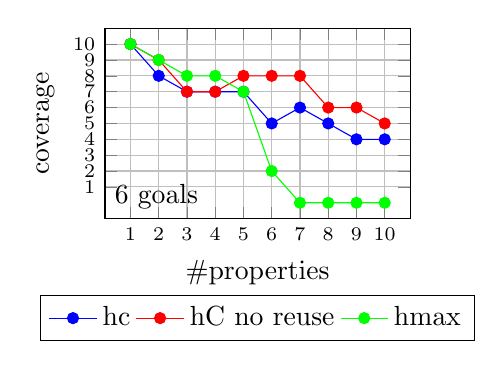
\begin{tikzpicture}
	\begin{axis}[
		title={6 goals},
		every axis title/.style={above right,at={(0,0)}},
		height=4cm,
		width=0.45\textwidth,
		xlabel=\#properties,
		ylabel=coverage,
		ytick={1,2,3,4,5,6,7,8,9,10},
		xtick={1,2,3,4,5,6,7,8,9,10},
		%xmin=0,
		%xmax=10,
		%ymin=0,
		%ymax=10,
		grid,
		%ybar,
		%bar width=2pt,
		legend style={at={(0.5,-0.4)}, anchor=north,legend columns=-1},
		%mark options={%
		%	scale=2,fill=yellow!80!black,draw=black
		%}
	]

	\addplot+[blue, mark=*, solid,mark options={fill=blue}] coordinates {
				(1,10) (2,8) (3,7) (4,7) (5,7) (6,5) (7,6) (8,5) (9,4) (10,4)
	};
	\addplot+[red, mark=*, mark options={fill=red}] coordinates {
				(1,10) (2,9) (3,7) (4,7) (5,8) (6,8) (7,8) (8,6) (9,6) (10,5)
	};
	\addplot+[green, mark=*, mark options={fill=green}] coordinates {
				(1,10) (2,9) (3,8) (4,8) (5,7) (6,2) (7,0) (8,0) (9,0) (10,0)
	};
	
	\legend{hc, hC no reuse, hmax}
	\end{axis}
\end{tikzpicture}
\caption{Nomystery domain with 2 trucks. Scale number of packages/goal facts between 2 and 6 and number of 
	properties between 1 and 10. The three property types blocked/forced road and two packages have
	to be delivered in the same truck are added in a fixed order. }
\end{figure}

\begin{figure}[ht]
\centering
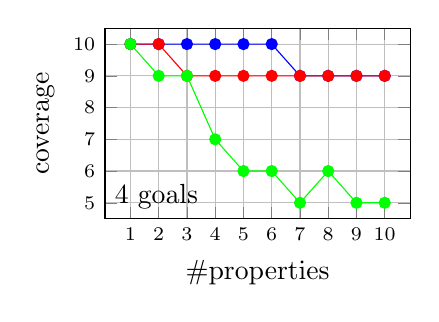
\begin{tikzpicture}
	\begin{axis}[
		title={4 goals},
		every axis title/.style={above right,at={(0,0)}},
		height=4cm,
		width=0.45\textwidth,
		xlabel=\#properties,
		ylabel=coverage,
		ytick={1,2,3,4,5,6,7,8,9,10},
		xtick={1,2,3,4,5,6,7,8,9,10},
		grid,
		legend style={at={(0.2,1.15)}, anchor=north,legend columns=-1},
	]
	\addplot+[blue,mark=*, mark options={fill=blue}] coordinates {
				(1,10) (2,10) (3,10) (4,10) (5,10) (6,10) (7,9) (8,9) (9,9) (10,9)
	};
	\addplot+[red,mark=*, mark options={fill=red}] coordinates {
				(1,10) (2,10) (3,9) (4,9) (5,9) (6,9) (7,9) (8,9) (9,9) (10,9)
	};
	\addplot+[green,mark=*, mark options={fill=green}] coordinates {
				(1,10) (2,9) (3,9) (4,7) (5,6) (6,6) (7,5) (8,6) (9,5) (10,5)
	};

	
	%\legend{hC, hC no reuse, hmax}
	\end{axis}
\end{tikzpicture}
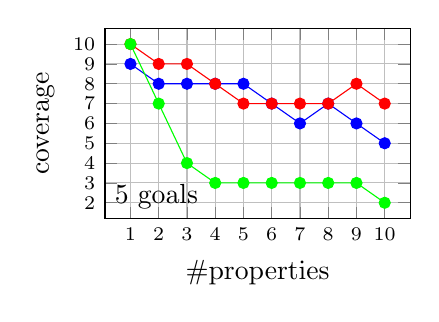
\begin{tikzpicture}
	\begin{axis}[
		title={5 goals},
		every axis title/.style={above right,at={(0,0)}},
		height=4cm,
		width=0.45\textwidth,
		xlabel=\#properties,
		ylabel=coverage,
		ytick={1,2,3,4,5,6,7,8,9,10},
		xtick={1,2,3,4,5,6,7,8,9,10},
		grid,
		legend style={at={(0.5,1.15)}, anchor=north,legend columns=-1},
	]
	\addplot+[blue, mark=*, mark options={fill=blue}] coordinates {
				(1,9) (2,8) (3,8) (4,8) (5,8) (6,7) (7,6) (8,7) (9,6) (10,5)
	};
	\addplot+[red, mark=*, mark options={fill=red}] coordinates {
				(1,10) (2,9) (3,9) (4,8) (5,7) (6,7) (7,7) (8,7) (9,8) (10,7)
	};
	\addplot+[green, mark=*, mark options={fill=green}] coordinates {
				(1,10) (2,7) (3,4) (4,3) (5,3) (6,3) (7,3) (8,3) (9,3) (10,2)
	};
	
	%\legend{hC, hC no reuse, hmax}
	\end{axis}
\end{tikzpicture}
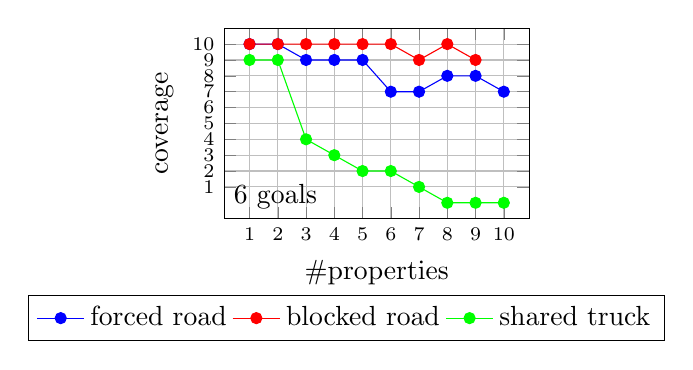
\begin{tikzpicture}
	\begin{axis}[
		title={6 goals},
		every axis title/.style={above right,at={(0,0)}},
		height=4cm,
		width=0.45\textwidth,
		xlabel=\#properties,
		ylabel=coverage,
		ytick={1,2,3,4,5,6,7,8,9,10},
		xtick={1,2,3,4,5,6,7,8,9,10},
		grid,
		legend style={at={(0.4,-0.4)}, anchor=north,legend columns=-1},
	]

	\addplot+[blue, mark=*, solid,mark options={fill=blue}] coordinates {
				(1,10) (2,10) (3,9) (4,9) (5,9) (6,7) (7,7) (8,8) (9,8) (10,7)
	};
	\addplot+[red, mark=*, mark options={fill=red}] coordinates {
				(1,10) (2,10) (3,10) (4,10) (5,10) (6,10) (7,9) (8,10) (9,9) 
	};
	\addplot+[green, mark=*, mark options={fill=green}] coordinates {
				(1,9) (2,9) (3,4) (4,3) (5,2) (6,2) (7,1) (8,0) (9,0) (10,0)
	};
	
	\legend{forced road, blocked road, shared truck}
	\end{axis}
\end{tikzpicture}
\caption{Nomystery domain with 2 trucks. Scale number of packages/goal facts between 2 and 6 and number of 
	properties between 1 and 10. For every combination of \#goals \#properties and property type 
	there are 10 instances. }
\end{figure}





\begin{figure}[ht]
\centering
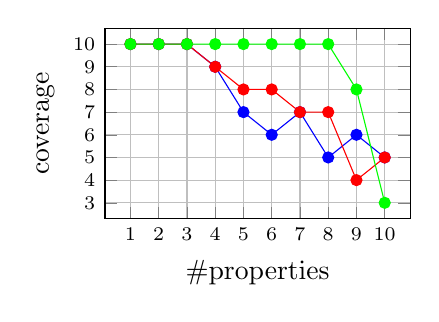
\begin{tikzpicture}
	\begin{axis}[
		height=4cm,
		width=0.45\textwidth,
		xlabel=\#properties,
		ylabel=coverage,
		ytick={1,2,3,4,5,6,7,8,9,10},
		xtick={1,2,3,4,5,6,7,8,9,10},
		%xmin=0,
		%xmax=10,
		%ymin=0,
		%ymax=10,
		grid,
		%ybar,
		%bar width=2pt,
		legend style={at={(0.5,1.15)}, anchor=north,legend columns=-1},
	]
				
	\addplot+[blue,mark=*, mark options={fill=blue}] coordinates {
				(1,10) (2,10) (3,10) (4,9) (5,7) (6,6) (7,7) (8,5) (9,6) (10,5)
	};
	\addplot+[red,mark=*, mark options={fill=red}] coordinates {
				(1,10) (2,10) (3,10) (4,9) (5,8) (6,8) (7,7) (8,7) (9,4) (10,5)
	};
	\addplot+[green,mark=*, mark options={fill=green}] coordinates {
				(1,10) (2,10) (3,10) (4,10) (5,10) (6,10) (7,10) (8,10) (9,8) (10,3)
	};

	%\legend{hC, hC no reuse, hmax}
	\end{axis}
\end{tikzpicture}
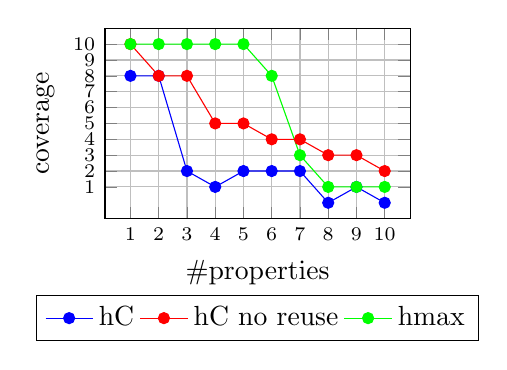
\begin{tikzpicture}
	\begin{axis}[
		height=4cm,
		width=0.45\textwidth,
		xlabel=\#properties,
		ylabel=coverage,
		ytick={1,2,3,4,5,6,7,8,9,10},
		xtick={1,2,3,4,5,6,7,8,9,10},
		%xmin=0,
		%xmax=10,
		%ymin=0,
		%ymax=10,
		grid,
		%ybar,
		%bar width=2pt,
		legend style={at={(0.5,-0.4)}, anchor=north,legend columns=-1},
	]

	\addplot+[blue, mark=*, mark options={fill=blue}] coordinates {
				(1,8) (2,8) (3,2) (4,1) (5,2) (6,2) (7,2) (8,0) (9,1) (10,0)
	};
	\addplot+[red, mark=*, mark options={fill=red}] coordinates {
				(1,10) (2,8) (3,8) (4,5) (5,5) (6,4) (7,4) (8,3) (9,3) (10,2)
	};
	\addplot+[green, mark=*, mark options={fill=green}] coordinates {
				(1,10) (2,10) (3,10) (4,10) (5,10) (6,8) (7,3) (8,1) (9,1) (10,1)
	};

	
	\legend{hC, hC no reuse, hmax}
	\end{axis}
\end{tikzpicture}
\caption{TPP domain with 2 trucks. Scale number of packages between 3 and 6 and number of 
	properties between 1 and 10. The three property types blocked/forced road and one goods needs to be bought a 
	specific market are added in a fixed order. }
\end{figure}

\begin{figure}[ht]
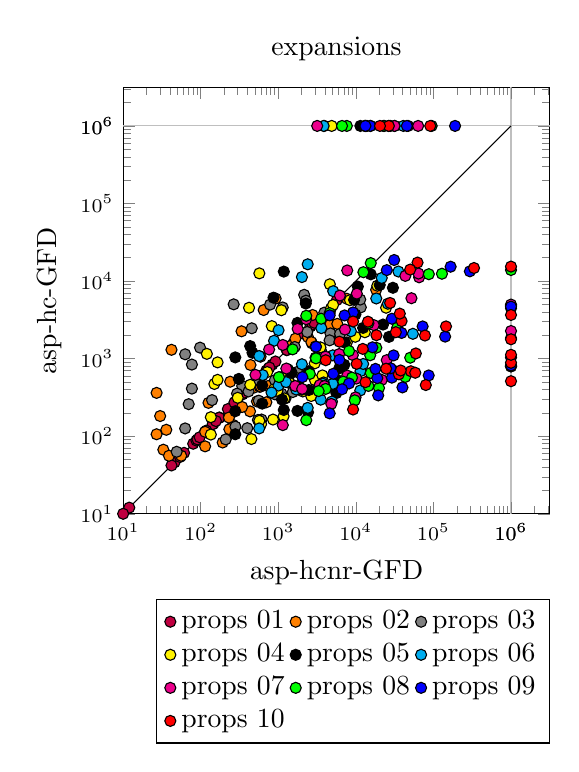
\begin{tikzpicture}
\begin{axis}[extra x tick style={grid=major}, extra x ticks=1000000, 
	extra y tick style={grid=major}, extra y ticks=1000000, height=7cm, 
	legend cell align=left, legend style={at={(1, -0.2)}, legend columns=3}, 
	title=expansions, width=7cm, xlabel=asp-hcnr-GFD, xmin=10, xmode=log, ylabel=asp-hc-GFD, ymin=10, ymode=log]
\addplot[color=purple, mark=*, mark options={{draw=black}}, only marks] coordinates {
(144, 144) (1557, 1557) (1286, 1286) (12, 12) (275, 275) (55, 55) (113, 113) (80, 80) (376, 376) (6268, 6268) (702, 702) (554, 554) (172, 172) (565, 565) (147, 147) (837, 837) (61, 61) (46, 46) (346, 346) (0.100000, 0.100000) (174, 174) (919, 919) (224, 224) (430, 430) (2946, 2946) (2104, 2104) (42, 42) (143, 143) (1472, 1472) (6362, 6362) (366, 366) (749, 749) (9, 9) (1292, 1292) (88, 88) (173, 173) (5691, 5691) (157, 157) (91, 91) (2595, 2595) (54, 54) (118, 118) (2761, 2761) (769, 769) (296, 296) (272, 272) (2910, 2910) (97, 97) (10, 10)
};
\addlegendentry{props 01}
\addplot[color=orange, mark=*, mark options={{draw=black}}, only marks] coordinates {
(432, 209) (2412, 1900) (648, 4233) (56, 56) (42, 1300) (930, 409) (30, 182) (4383, 2877) (261, 140) (0.100000, 205) (531, 281) (234, 123) (114, 114) (4671, 2740) (438, 828) (591, 1061) (738, 443) (1473, 1473) (3918, 1000000) (231, 174) (387, 407) (489, 424) (924, 5952) (0.100000, 173) (342, 238) (2715, 1575) (27, 106) (33, 67) (36, 121) (240, 504) (7674, 5907) (2769, 3652) (336, 2252) (702, 274) (27, 362) (1000000, 1840) (5763, 2807) (192, 83) (39, 56) (576, 434) (18267, 7725) (126, 269) (594, 437) (1662, 1809) (2673, 1632) (1050, 569) (114, 74)
};
\addlegendentry{props 02}
\addplot[color=gray, mark=*, mark options={{draw=black}}, only marks] coordinates {
(4704, 2113) (560, 287) (903, 347) (280, 133) (140, 292) (1547, 436) (63, 126) (77, 411) (784, 4973) (1141, 4568) (1239, 308) (4585, 1723) (63, 1138) (1099, 354) (343, 445) (98, 1387) (399, 127) (2156, 6648) (3570, 1254) (11578, 4584) (455, 2462) (77, 839) (6258, 2089) (2359, 2208) (210, 91) (3919, 3919) (11389, 5776) (560, 529) (1540, 371) (266, 5011) (2275, 5588) (609, 164) (1386, 503) (0.100000, 195) (49, 63) (413, 378) (0.100000, 59) (0.100000, 282) (1631, 1413) (70, 259) (294, 354) (1757, 674) (546, 162) (903, 528)
};
\addlegendentry{props 03}
\addplot[color=yellow, mark=*, mark options={{draw=black}}, only marks] coordinates {
(1095, 4212) (18900, 8717) (885, 404) (165, 895) (150, 472) (0.100000, 345) (8400, 5672) (600, 143) (420, 4528) (570, 12572) (0.100000, 266) (120, 1153) (2970, 528) (1200, 307) (720, 671) (7650, 1618) (24540, 4534) (2655, 330) (1170, 181) (825, 2627) (4770, 4433) (9825, 1914) (4875, 1000000) (300, 313) (0.100000, 71) (435, 460) (4620, 9099) (1200, 596) (3495, 1398) (5085, 4922) (2955, 870) (855, 164) (13050, 2190) (450, 92) (2070, 378) (975, 384) (0.100000, 209) (1335, 526) (3705, 608) (570, 158) (135, 176) (165, 533) (135, 105)
};
\addlegendentry{props 04}
\addplot[color=black, mark=*, mark options={{draw=black}}, only marks] coordinates {
(1178, 218) (13175, 1000000) (1178, 13248) (0.100000, 621) (868, 6106) (5642, 533) (4278, 422) (7223, 1606) (22413, 2751) (2418, 203) (1829, 444) (2263, 5137) (26753, 1909) (9858, 3709) (2015, 398) (279, 106) (20305, 8903) (620, 263) (1333, 727) (12400, 2493) (15562, 12215) (1767, 2891) (434, 1451) (279, 210) (1767, 212) (2480, 688) (465, 1190) (2480, 394) (1116, 297) (6107, 748) (620, 454) (11439, 1000000) (30039, 8195) (279, 1038) (7099, 833) (0.100000, 133) (0.100000, 257) (15500, 1000000) (310, 548) (10602, 8487) (0.100000, 88) (5611, 360) (0.100000, 432) (9486, 5730) (1488, 658)
};
\addlegendentry{props 05}
\addplot[color=cyan, mark=*, mark options={{draw=black}}, only marks] coordinates {
(3339, 433) (1701, 400) (0.100000, 486) (35343, 13277) (630, 614) (5040, 473) (13860, 1000000) (2016, 11258) (11403, 389) (567, 1080) (21546, 10963) (1008, 450) (8631, 2254) (54369, 2090) (25830, 5102) (3591, 2473) (0.100000, 731) (2016, 847) (2394, 16457) (3024, 1436) (18333, 5966) (3528, 296) (3843, 1000000) (40950, 1000000) (1008, 2326) (3024, 1031) (0.100000, 474) (1000000, 4830) (567, 126) (882, 1699) (0.100000, 154) (11466, 689) (2394, 232) (1260, 498) (4914, 280) (3843, 493) (819, 366) (13104, 1000000) (23247, 1000000) (5103, 7403) (5040, 1102) (0.100000, 163) (31500, 1000000) (3717, 477) (12411, 854)
};
\addlegendentry{props 06}
\addplot[color=magenta, mark=*, mark options={{draw=black}}, only marks] coordinates {
(7493, 510) (0.100000, 192) (1651, 444) (4826, 261) (0.100000, 473) (1143, 139) (6223, 6507) (0.100000, 299) (7239, 2370) (3429, 457) (27940, 1000000) (43434, 11665) (762, 1312) (2286, 3224) (2032, 407) (7747, 13704) (9906, 317) (9144, 1112) (6096, 1146) (3937, 444) (0.100000, 718) (0.100000, 611) (1270, 746) (7112, 485) (1000000, 2271) (1778, 2422) (1000000, 4977) (10160, 553) (52070, 6012) (10287, 6890) (31496, 1000000) (3175, 1000000) (65405, 11183) (17018, 2707) (25019, 957) (21590, 532) (64135, 12513) (1000000, 793) (1143, 1501) (508, 618) (47117, 1000000) (26416, 1000000) (4064, 1062) (7747, 605) (63500, 1000000)
};
\addlegendentry{props 07}
\addplot[color=green, mark=*, mark options={{draw=black}}, only marks] coordinates {
(1000000, 799) (7650, 1000000) (19890, 418) (15555, 17047) (2295, 161) (22695, 1000000) (3060, 1009) (0.100000, 866) (1000000, 13893) (0.100000, 251) (6630, 1000000) (87210, 12266) (2550, 635) (8925, 570) (4080, 407) (9690, 290) (15300, 1106) (3570, 3272) (14535, 445) (0.100000, 962) (0.100000, 695) (1000000, 4472) (12495, 13014) (2295, 3568) (18360, 1382) (34170, 2517) (8160, 1255) (1020, 578) (50235, 1029) (30090, 707) (15555, 654) (14535, 2862) (0.100000, 269) (43350, 581) (6885, 505) (1530, 1317) (4590, 3866) (0.100000, 1637) (128775, 12433) (94860, 1000000) (3315, 382)
};
\addlegendentry{props 08}
\addplot[color=blue, mark=*, mark options={{draw=black}}, only marks] coordinates {
(9198, 3946) (15330, 1000000) (8176, 479) (38836, 2145) (4599, 197) (3066, 1425) (45479, 1000000) (19418, 336) (0.100000, 300) (86870, 607) (16352, 1399) (39858, 426) (166586, 15317) (4599, 3621) (13286, 1000000) (0.100000, 1875) (29127, 569) (30660, 1101) (18907, 561) (17885, 738) (31171, 18691) (0.100000, 957) (25039, 13840) (1000000, 819) (0.100000, 239) (28105, 751) (141547, 1923) (0.100000, 881) (2044, 578) (6132, 964) (1000000, 4683) (72562, 2602) (0.100000, 1921) (7154, 3606) (6643, 403) (294847, 13362) (29127, 3268) (1000000, 1037) (190092, 1000000) (5110, 638)
};
\addlegendentry{props 09}
\addplot[color=red, mark=*, mark options={{draw=black}}, only marks] coordinates {
(27621, 5220) (51150, 688) (1000000, 15370) (10230, 857) (58311, 658) (32736, 2193) (91047, 1000000) (79794, 457) (0.100000, 1630) (38874, 3047) (4092, 954) (333498, 14739) (12276, 1335) (0.100000, 917) (36828, 3806) (62403, 17312) (26598, 1000000) (1000000, 512) (24552, 742) (9207, 3015) (0.100000, 252) (1000000, 1777) (77748, 1986) (6138, 1655) (1000000, 3658) (35805, 628) (13299, 497) (0.100000, 301) (1000000, 885) (1000000, 1120) (14322, 2997) (20460, 1000000) (50127, 14064) (145266, 2602) (37851, 704) (0.100000, 1946) (9207, 221) (0.100000, 944) (18414, 2004) (59334, 1167)
};
\addlegendentry{props 10}
\addplot[color=black] coordinates {(0.050000, 0.050000) (1000000, 1000000)};
\end{axis}
\end{tikzpicture}

\input{data/action_set_properties/scatterplot-search_time_C-Cnr_GFD.tex}
\caption{nomystery}
\end{figure}



\begin{figure}[ht]
%\input{data/action_set_properties/scatterplot-expansions_C-Cnr_tpp_goals.tex}
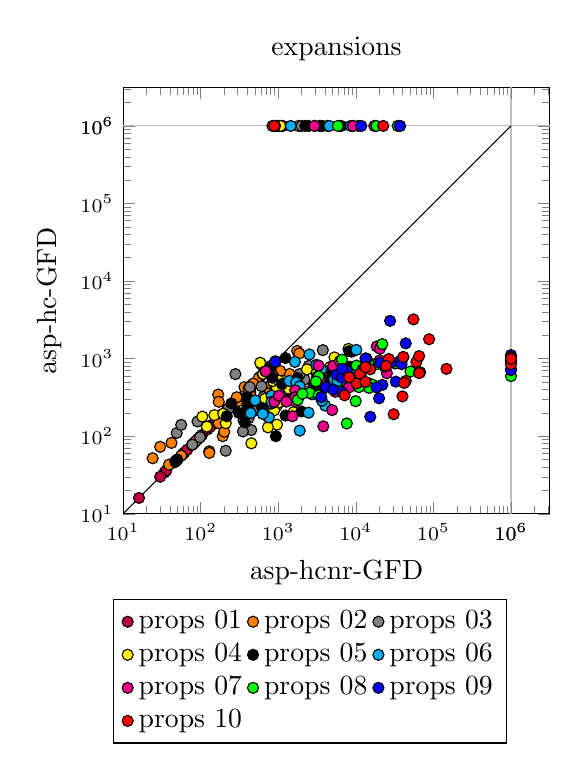
\begin{tikzpicture}
\begin{axis}[extra x tick style={grid=major}, extra x ticks=1000000, 
		extra y tick style={grid=major}, extra y ticks=1000000, height=7cm, 
		legend cell align=left, legend style={at={(0.9, -0.2)}, legend columns=3}, 
		title=expansions, width=7cm, xlabel=asp-hcnr-GFD, xmin=10, xmode=log, 
		ylabel=asp-hc-GFD, ymin=10, ymode=log]
\addplot[color=purple, mark=*, mark options={{draw=black}}, only marks] coordinates {
(220, 220) (85, 85) (122, 122) (428, 428) (313, 313) (631, 631) (16, 16) (92, 92) (141, 141) (59, 59) (46, 46) (570, 570) (1146, 1000000) (168, 168) (285, 285) (62, 62) (104, 104) (79, 79) (192, 192) (577, 577) (50, 50) (455, 455) (99, 99) (67, 67) (973, 1000000) (475, 475) (34, 34) (271, 271) (757, 757) (131, 131) (221, 221) (758, 758) (36, 36) (183, 183) (305, 305) (8, 8) (30, 30) (711, 711)
};
\addlegendentry{props 01}
\addplot[color=orange, mark=*, mark options={{draw=black}}, only marks] coordinates {
(1752, 1257) (168, 344) (77, 77) (207, 153) (184, 184) (435, 369) (366, 429) (42, 82) (306, 285) (56, 56) (855, 607) (192, 100) (129, 64) (435, 341) (1398, 635) (201, 114) (414, 262) (171, 147) (24, 52) (759, 403) (1000000, 735) (556, 556) (82, 82) (812, 812) (171, 278) (291, 318) (39, 43) (227, 227) (813, 470) (1863, 1167) (86, 86) (30, 73) (476, 476) (1059, 692) (632, 632) (414, 414) (129, 61) (47, 47) (1824, 1000000)
};
\addlegendentry{props 02}
\addplot[color=gray, mark=*, mark options={{draw=black}}, only marks] coordinates {
(2177, 539) (448, 120) (1995, 1000000) (735, 180) (840, 1000000) (350, 115) (3717, 1000000) (210, 65) (609, 441) (966, 294) (2933, 1000000) (636, 636) (434, 251) (2457, 1000000) (357, 160) (78, 78) (49, 110) (399, 279) (1421, 481) (48, 48) (413, 170) (483, 212) (399, 223) (98, 97) (847, 614) (2401, 742) (91, 155) (1015, 371) (1897, 635) (56, 140) (2471, 808) (228, 228) (280, 632) (3752, 1287) (430, 430) (1027, 1000000) (903, 445) (644, 321)
};
\addlegendentry{props 03}
\addplot[color=yellow, mark=*, mark options={{draw=black}}, only marks] coordinates {
(960, 417) (960, 248) (120, 133) (1065, 1000000) (4665, 781) (2340, 727) (885, 216) (4275, 1000000) (637, 637) (1020, 272) (960, 141) (2160, 379) (735, 130) (105, 179) (49, 49) (600, 851) (8040, 1335) (150, 187) (585, 885) (210, 147) (450, 81) (195, 195) (3120, 651) (645, 247) (6210, 1000000) (3390, 1000000) (1575, 204) (1380, 407) (855, 514) (1020, 520) (2070, 361) (4065, 679) (675, 304) (5295, 1038)
};
\addlegendentry{props 04}
\addplot[color=black, mark=*, mark options={{draw=black}}, only marks] coordinates {
(1333, 302) (806, 769) (1240, 185) (4836, 694) (1798, 365) (403, 245) (8401, 786) (2232, 1000000) (10726, 1000000) (1116, 471) (1984, 209) (1767, 563) (50, 50) (3348, 494) (372, 151) (2852, 454) (620, 231) (1240, 1017) (403, 313) (310, 200) (8866, 1231) (8184, 1248) (3503, 1000000) (248, 264) (3627, 388) (919, 919) (837, 568) (930, 100) (6479, 1000000) (3906, 534) (686, 686) (217, 181) (403, 235)
};
\addlegendentry{props 05}
\addplot[color=cyan, mark=*, mark options={{draw=black}}, only marks] coordinates {
(7371, 464) (917, 917) (5229, 537) (4032, 248) (1449, 1000000) (9828, 752) (7938, 579) (10143, 1298) (4536, 1000000) (3654, 287) (441, 199) (819, 333) (1638, 908) (756, 175) (2457, 201) (1386, 517) (630, 194) (17073, 841) (819, 263) (3591, 729) (1701, 495) (504, 290) (1890, 440) (5796, 513) (2520, 1131) (819, 277) (9198, 1000000) (8568, 1000000) (2709, 347) (3087, 831) (1890, 118) (687, 687)
};
\addlegendentry{props 06}
\addplot[color=magenta, mark=*, mark options={{draw=black}}, only marks] coordinates {
(5461, 374) (1651, 281) (25146, 649) (3429, 534) (14859, 477) (889, 278) (10541, 565) (18542, 1436) (3810, 134) (20320, 949) (1651, 390) (9144, 1000000) (5080, 804) (20447, 1343) (11684, 584) (1651, 318) (688, 688) (7239, 736) (6223, 928) (4953, 217) (2921, 1000000) (1016, 334) (3175, 586) (1000000, 934) (7366, 398) (1270, 279) (918, 918) (1524, 181) (17272, 1000000) (16002, 801) (8128, 424) (3302, 816)
};
\addlegendentry{props 07}
\addplot[color=green, mark=*, mark options={{draw=black}}, only marks] coordinates {
(910, 1000000) (18870, 852) (16320, 462) (1000000, 596) (14535, 861) (21930, 1538) (6630, 969) (18360, 1000000) (6885, 615) (23460, 790) (50490, 682) (2550, 362) (6120, 610) (14790, 420) (13770, 999) (40800, 1044) (3315, 590) (1785, 295) (10200, 814) (9945, 283) (5865, 1000000) (2040, 352) (37230, 1000000) (34680, 1000000) (3315, 337) (3060, 508) (32130, 867) (10965, 429) (7650, 146)
};
\addlegendentry{props 08}
\addplot[color=blue, mark=*, mark options={{draw=black}}, only marks] coordinates {
(5621, 622) (67452, 667) (15330, 178) (12264, 726) (43946, 1574) (6643, 568) (4088, 429) (19929, 308) (20440, 883) (29127, 896) (36792, 1000000) (32704, 505) (3577, 319) (5110, 399) (37814, 942) (13286, 1008) (6643, 369) (11753, 1000000) (7665, 694) (21973, 459) (1000000, 711) (1000000, 1112) (1000000, 949) (1000000, 1021) (18396, 426) (911, 911) (6643, 737) (38836, 849) (27594, 3068)
};
\addlegendentry{props 09}
\addplot[color=red, mark=*, mark options={{draw=black}}, only marks] coordinates {
(7161, 337) (87978, 1779) (30690, 192) (43989, 516) (1000000, 877) (65472, 663) (10230, 478) (60357, 910) (8184, 575) (1000000, 1045) (15345, 729) (1000000, 848) (147312, 738) (11253, 638) (65472, 650) (41943, 486) (13299, 500) (55242, 3208) (1000000, 994) (40920, 1051) (13299, 779) (39897, 326) (26598, 990) (889, 1000000) (24552, 806) (22506, 1000000) (65472, 1079)
};
\addlegendentry{props 10}
\addplot[color=black] coordinates {(0.050000, 0.050000) (1000000, 1000000)};
\end{axis}
\end{tikzpicture}

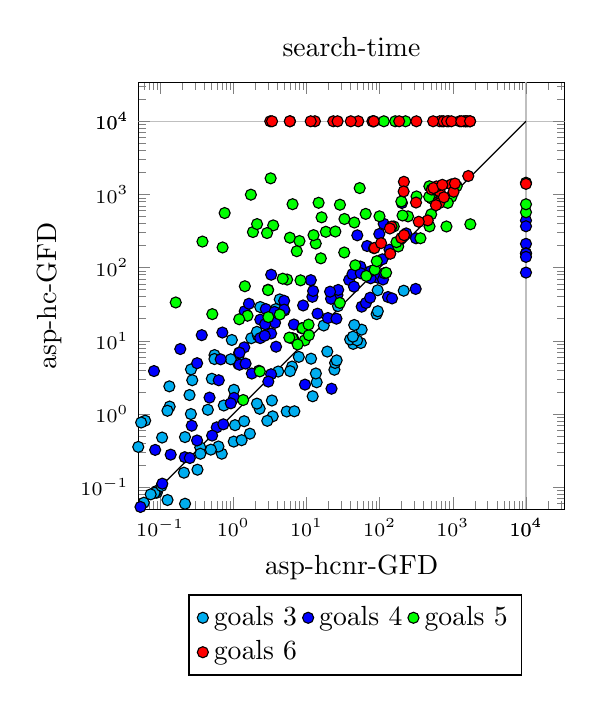
\begin{tikzpicture}
\begin{axis}[extra x tick style={grid=major}, extra x ticks=10000, 
	extra y tick style={grid=major}, extra y ticks=10000, height=7cm, 
	legend cell align=left, legend style={at={(0.9, -0.2)}, legend columns=3}, 
	title=search-time, width=7cm, xlabel=asp-hcnr-GFD, xmin=0.05, xmode=log, ylabel=asp-hc-GFD, ymin=0.05, ymode=log]
\addplot[color=cyan, mark=*, mark options={{draw=black}}, only marks] coordinates {
(0.012686, 0.018468) (13.777100, 2.710320) (19.240200, 7.120620) (0.090099, 0.083997) (2.235020, 3.897000) (0.218968, 0.059241) (43.474200, 9.070310) (5.364710, 1.079980) (0.051041, 0.048613) (2.290610, 1.176320) (0.741274, 1.304950) (24.066500, 4.017910) (1.055250, 0.702632) (6.354300, 4.442340) (90.877300, 23.160200) (93.913600, 49.026600) (0.047240, 0.032462) (0.263980, 4.060410) (0.087937, 0.087912) (1.684110, 0.537619) (1.758720, 10.837800) (0.010000, 0.010000) (0.323599, 0.172992) (0.694918, 0.286133) (0.011962, 0.196532) (0.625814, 0.359063) (0.109042, 0.049356) (4.109860, 3.801110) (2.334540, 28.923300) (213.176000, 48.347800) (39.496600, 10.410300) (26.936400, 29.782600) (1.013270, 0.418749) (3.455810, 0.927333) (0.059770, 0.061135) (1.168960, 6.025890) (6.826830, 1.087410) (0.553401, 6.379160) (0.353499, 0.348109) (1.169700, 4.838980) (0.263053, 0.997536) (0.028932, 0.029786) (5.971980, 3.843950) (2.167970, 11.815100) (2.911860, 0.805406) (0.026584, 0.027641) (0.211461, 0.157457) (0.448392, 1.140220) (24.607800, 4.980320) (1.298650, 0.438021) (55.213600, 9.320400) (0.218497, 0.482936) (0.010861, 0.011967) (0.039108, 0.038952) (49.164400, 10.147900) (94.361600, 25.345400) (56.719400, 14.195200) (4.313840, 36.791700) (0.274739, 2.889950) (1.019290, 2.138070) (0.106340, 0.475902) (0.024822, 0.028767) (0.012186, 0.010000) (0.134875, 1.261720) (0.133598, 2.382330) (0.126099, 0.066667) (0.027139, 0.026656) (0.029112, 0.745081) (17.217100, 16.190800) (3.814990, 27.108400) (0.062388, 0.809774) (2.102800, 1.384390) (3.366070, 1.527520) (44.927300, 16.432900) (0.054971, 0.763861) (0.083944, 0.083588) (12.149900, 1.744320) (25.847500, 5.399750) (0.954348, 10.254100) (0.031984, 0.967532) (11.546400, 5.693150) (0.041545, 0.043900) (0.508750, 3.028120) (0.011869, 0.012096) (0.552349, 5.633040) (1.405690, 0.795521) (0.492758, 0.325301) (13.434200, 3.575160) (0.922851, 5.591520) (0.104341, 0.103738) (0.125756, 1.105880) (0.028317, 0.028907) (7.848800, 6.027390) (43.094800, 11.387100) (0.010043, 0.108707) (0.050231, 0.354371) (0.252034, 1.813100) (0.354536, 0.285740) (2.103460, 13.249500) (0.074183, 0.079645)
};
\addlegendentry{goals 3}
\addplot[color=blue, mark=*, mark options={{draw=black}}, only marks] coordinates {
(0.593416, 0.655578) (4.991990, 25.909400) (94.670600, 72.712200) (0.708234, 12.965200) (10000, 439.668000) (111.087000, 68.821400) (3.286660, 12.576600) (38.302300, 67.667400) (0.217147, 0.256366) (24.351700, 40.338200) (136.530000, 175.756000) (0.188454, 7.713660) (0.106920, 0.111535) (10000, 85.518600) (14.161500, 23.475500) (230.472000, 293.598000) (1.431430, 25.373300) (0.020963, 1.130940) (0.254451, 0.249715) (0.043534, 0.125005) (0.730083, 0.721303) (12.048000, 39.922500) (2.336390, 19.454400) (0.671829, 5.578140) (1.635800, 32.079800) (54.536700, 103.330000) (10000, 211.323000) (19.628600, 20.478900) (0.320074, 4.939490) (3.840790, 8.301850) (49.498200, 276.354000) (21.986800, 2.212290) (2.331500, 10.879500) (9.540610, 2.516980) (313.156000, 251.765000) (2.779630, 27.132800) (0.473147, 1.672130) (56.836500, 29.249000) (0.010000, 0.010000) (26.462800, 42.109600) (0.319681, 0.433884) (0.010000, 0.099429) (64.978900, 32.843100) (4.947870, 35.195900) (3.293050, 79.948600) (1.410290, 8.130530) (115.646000, 84.004400) (10000, 157.252000) (8.620140, 14.828600) (10000, 155.684000) (130.014000, 39.685500) (3.657250, 24.808200) (42.461900, 81.394200) (1.790710, 3.568160) (1.215490, 4.708270) (1.202190, 6.895400) (75.287900, 71.494200) (0.270100, 0.690682) (6.733820, 16.688000) (10000, 140.195000) (74.105300, 38.812500) (27.131800, 49.541900) (113.485000, 397.455000) (12.313300, 47.950600) (75.186800, 89.215700) (98.904900, 288.281000) (1.217140, 6.863820) (310.755000, 51.155700) (0.513277, 0.506373) (0.053864, 0.053605) (147.762000, 37.935500) (0.632161, 2.886310) (55.128500, 83.671800) (21.661800, 37.521400) (21.004000, 46.895400) (108.923000, 129.789000) (3.720920, 17.624200) (6.588940, 10.738000) (3.281640, 3.489010) (10000, 367.569000) (0.018648, 0.119977) (0.370328, 11.936300) (0.139223, 0.277867) (2.685970, 11.736100) (0.082363, 3.856860) (2.720190, 16.847800) (1.022730, 1.658470) (3.008850, 2.767970) (0.085493, 0.322556) (11.453000, 67.369300) (67.396500, 197.516000) (8.995970, 30.391500) (0.044703, 1.426120) (0.923861, 1.397460) (83.595100, 184.298000) (44.591600, 54.930500) (25.673600, 20.051800) (4.948640, 26.655400) (201.609000, 763.914000) (1.471410, 4.876470)
};
\addlegendentry{goals 4}
\addplot[color=green, mark=*, mark options={{draw=black}}, only marks] coordinates {
(65.699500, 76.973500) (33.029700, 462.106000) (1.852760, 306.413000) (85.545600, 93.564900) (710.068000, 10000) (10000, 571.317000) (0.713880, 188.591000) (512.504000, 879.127000) (8.294470, 66.970100) (13.385700, 213.494000) (4.316110, 22.851000) (45.032200, 413.287000) (83.375100, 10000) (360.932000, 251.963000) (18.393700, 308.729000) (10000, 734.552000) (1735.270000, 391.493000) (3.010810, 21.065000) (9.445270, 10.116500) (12.485100, 277.765000) (179.289000, 194.451000) (5.439540, 68.688500) (163.069000, 10000) (0.163415, 33.392300) (0.761220, 556.889000) (16.085900, 486.712000) (197.937000, 802.118000) (28.660700, 723.484000) (0.378776, 226.852000) (1414.390000, 10000) (3.509460, 377.575000) (7.364590, 167.650000) (91.394800, 122.391000) (8.840550, 14.874200) (14.642700, 769.436000) (32.797700, 160.973000) (6.374390, 10.832400) (28.544300, 32.917700) (1.562870, 21.993700) (1.204740, 19.694200) (10.772200, 11.929500) (506.075000, 535.652000) (225.421000, 10000) (2.989640, 49.866800) (1.437750, 55.656500) (122.575000, 85.186200) (477.826000, 1293.500000) (169.694000, 222.926000) (2.889180, 296.792000) (1130.330000, 1300.800000) (818.041000, 364.843000) (956.134000, 928.888000) (1.737950, 992.840000) (5.931930, 256.310000) (8.019290, 230.953000) (480.645000, 365.696000) (99.482500, 502.377000) (10000, 1446.680000) (852.304000, 766.589000) (15.696900, 133.887000) (6.452530, 735.922000) (0.516290, 23.136000) (319.536000, 939.201000) (7.574030, 8.905050) (46.415000, 107.579000) (474.571000, 927.586000) (4.733110, 70.585300) (24.803800, 311.645000) (3.235740, 1660.440000) (244.168000, 501.494000) (2.299860, 3.816750) (114.088000, 10000) (2.981500, 49.288800) (5.825620, 11.045300) (10.680400, 16.646200) (205.580000, 515.996000) (53.353900, 1221.450000) (156.032000, 365.378000) (64.458200, 542.436000) (1.364070, 1.549990) (2.111470, 393.522000)
};
\addlegendentry{goals 5}
\addplot[color=red, mark=*, mark options={{draw=black}}, only marks] coordinates {
(13.033600, 10000) (185.057000, 10000) (197.682000, 254.174000) (23.245500, 10000) (879.000000, 10000) (630.051000, 786.688000) (662.202000, 10000) (50.998800, 10000) (748.435000, 10000) (5.962050, 10000) (1492.600000, 10000) (3.196190, 10000) (453.890000, 441.892000) (79.578700, 10000) (3.381850, 10000) (215.517000, 277.873000) (85.088300, 185.556000) (26.615600, 10000) (1723.770000, 10000) (314.205000, 775.662000) (1240.110000, 10000) (317.620000, 10000) (956.424000, 1372.160000) (145.371000, 363.671000) (137.854000, 342.459000) (1024.040000, 1087.160000) (139.634000, 154.579000) (342.210000, 423.418000) (1604.330000, 10000) (10000, 1395.500000) (104.695000, 215.797000) (834.167000, 10000) (214.339000, 1489.210000) (40.341700, 10000) (956.087000, 10000) (514.427000, 1167.470000) (659.598000, 1103.580000) (649.701000, 758.802000) (596.676000, 1286.690000) (544.156000, 1223.120000) (537.926000, 10000) (1517.460000, 10000) (1626.110000, 1786.550000) (82.827300, 10000) (212.711000, 1098.330000) (5.911980, 10000) (588.183000, 712.668000) (11.427400, 10000) (1306.220000, 10000) (718.448000, 1353.800000) (754.553000, 914.113000) (1718.960000, 10000) (1068.970000, 1410.650000)
};
\addlegendentry{goals 6}
\addplot[color=black] coordinates {(0.050000, 0.050000) (10000, 10000)};
\end{axis}
\end{tikzpicture}

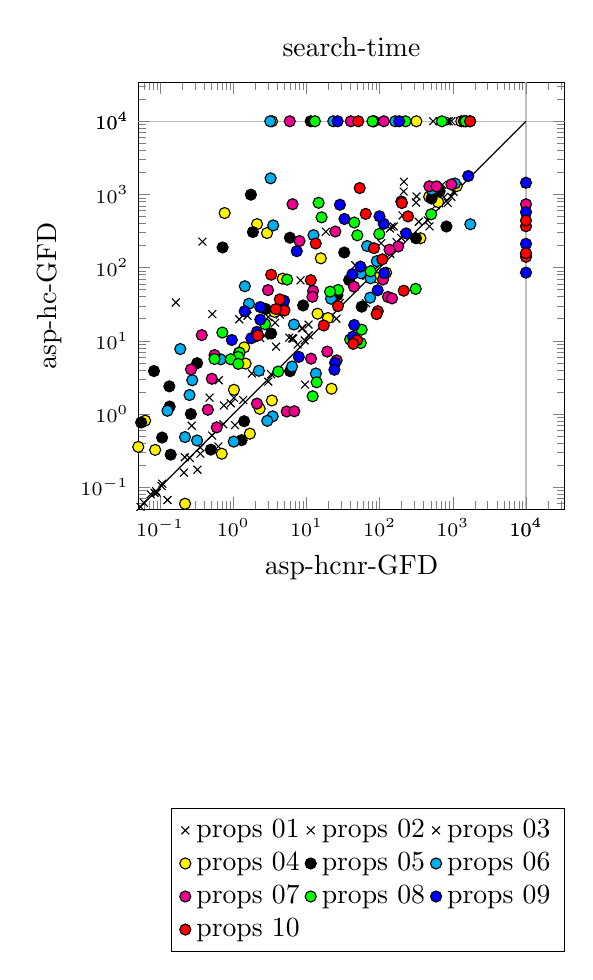
\begin{tikzpicture}
\begin{axis}[extra x tick style={grid=major}, extra x ticks=10000, 
	extra y tick style={grid=major}, extra y ticks=10000,
	height=7cm, legend cell align=left, legend style={at={(1.0, -0.7)}, legend columns=3}, title=search-time, width=7cm, xlabel=asp-hcnr-GFD, xmin=0.05, xmode=log, ylabel=asp-hc-GFD, ymin=0.05, ymode=log]
\addplot[color=blue, mark=x, mark options={{draw=black}}, only marks] coordinates {
(65.699500, 76.973500) (3.281640, 3.489010) (85.545600, 93.564900) (197.682000, 254.174000) (215.517000, 277.873000) (1.790710, 3.568160) (0.090099, 0.083997) (0.010861, 0.011967) (137.854000, 342.459000) (453.890000, 441.892000) (1604.330000, 10000) (0.217147, 0.256366) (9.445270, 10.116500) (1.022730, 1.658470) (0.011869, 0.012096) (0.051041, 0.048613) (8.840550, 14.874200) (0.059770, 0.061135) (28.544300, 32.917700) (0.106920, 0.111535) (139.634000, 154.579000) (0.039108, 0.038952) (0.513277, 0.506373) (0.053864, 0.053605) (956.087000, 10000) (0.012186, 0.010000) (0.923861, 1.397460) (7.574030, 8.905050) (0.730083, 0.721303) (1024.040000, 1087.160000) (0.027139, 0.026656) (2.299860, 3.816750) (588.183000, 712.668000) (5.825620, 11.045300) (10.680400, 16.646200) (718.448000, 1353.800000) (0.010000, 0.010000) (1.364070, 1.549990) (0.074183, 0.079645)
};
\addlegendentry{props 01}
\addplot[color=red, mark=x, mark options={{draw=black}}, only marks] coordinates {
(3.720920, 17.624200) (0.012686, 0.018468) (0.018648, 0.119977) (314.205000, 775.662000) (480.645000, 365.696000) (3.840790, 8.301850) (2.685970, 11.736100) (3.010810, 21.065000) (748.435000, 10000) (0.163415, 33.392300) (10.772200, 11.929500) (0.041545, 0.043900) (25.673600, 20.051800) (85.088300, 185.556000) (0.270100, 0.690682) (10000, 1395.500000) (145.371000, 363.671000) (3.008850, 2.767970) (0.473147, 1.672130) (1.562870, 21.993700) (0.516290, 23.136000) (8.294470, 66.970100) (342.210000, 423.418000) (0.353499, 0.348109) (0.104341, 0.103738) (214.339000, 1489.210000) (0.254451, 0.249715) (0.010000, 0.099429) (0.047240, 0.032462) (319.536000, 939.201000) (46.415000, 107.579000) (0.087937, 0.087912) (212.711000, 1098.330000) (156.032000, 365.378000) (0.126099, 0.066667) (0.026584, 0.027641) (0.010043, 0.108707) (754.553000, 914.113000) (0.211461, 0.157457)
};
\addlegendentry{props 02}
\addplot[color=green, mark=x, mark options={{draw=black}}, only marks] coordinates {
(6.588940, 10.738000) (0.011962, 0.196532) (0.083944, 0.083588) (879.000000, 10000) (0.625814, 0.359063) (18.393700, 308.729000) (1.215490, 4.708270) (662.202000, 10000) (0.109042, 0.049356) (5.962050, 10000) (0.323599, 0.172992) (64.978900, 32.843100) (2.331500, 10.879500) (1240.110000, 10000) (9.540610, 2.516980) (1.204740, 19.694200) (0.741274, 1.304950) (1.055250, 0.702632) (6.374390, 10.832400) (0.020963, 1.130940) (0.024822, 0.028767) (104.695000, 215.797000) (852.304000, 766.589000) (956.134000, 928.888000) (4.316110, 22.851000) (649.701000, 758.802000) (169.694000, 222.926000) (24.351700, 40.338200) (537.926000, 10000) (0.632161, 2.886310) (2.989640, 49.866800) (0.043534, 0.125005) (0.029112, 0.745081) (8.620140, 14.828600) (205.580000, 515.996000) (0.354536, 0.285740) (834.167000, 10000) (0.378776, 226.852000)
};
\addlegendentry{props 03}
\addplot[color=yellow, mark=*, mark options={{draw=black}}, only marks] coordinates {
(0.694918, 0.286133) (3.657250, 24.808200) (3.366070, 1.527520) (94.670600, 72.712200) (19.628600, 20.478900) (630.051000, 786.688000) (0.031984, 0.967532) (3.381850, 10000) (0.761220, 556.889000) (1306.220000, 10000) (21.986800, 2.212290) (1723.770000, 10000) (2.290610, 1.176320) (317.620000, 10000) (122.575000, 85.186200) (0.085493, 0.322556) (14.161500, 23.475500) (1.019290, 2.138070) (0.218968, 0.059241) (0.044703, 1.426120) (1130.330000, 1300.800000) (2.111470, 393.522000) (15.696900, 133.887000) (474.571000, 927.586000) (4.733110, 70.585300) (1.410290, 8.130530) (0.028317, 0.028907) (2.889180, 296.792000) (360.932000, 251.963000) (1.684110, 0.537619) (4.948640, 26.655400) (0.050231, 0.354371) (0.062388, 0.809774) (1.471410, 4.876470)
};
\addlegendentry{props 04}
\addplot[color=black, mark=*, mark options={{draw=black}}, only marks] coordinates {
(659.598000, 1103.580000) (1.852760, 306.413000) (1.298650, 0.438021) (0.054971, 0.763861) (0.320074, 4.939490) (3.286660, 12.576600) (38.302300, 67.667400) (0.082363, 3.856860) (5.931930, 256.310000) (1414.390000, 10000) (313.156000, 251.765000) (32.797700, 160.973000) (512.504000, 879.127000) (1.405690, 0.795521) (5.971980, 3.843950) (0.492758, 0.325301) (0.139223, 0.277867) (56.836500, 29.249000) (8.995970, 30.391500) (0.263053, 0.997536) (0.106340, 0.475902) (26.462800, 42.109600) (544.156000, 1223.120000) (0.028932, 0.029786) (818.041000, 364.843000) (2.779630, 27.132800) (0.134875, 1.261720) (0.133598, 2.382330) (82.827300, 10000) (0.713880, 188.591000) (11.427400, 10000) (1517.460000, 10000) (1.737950, 992.840000)
};
\addlegendentry{props 05}
\addplot[color=cyan, mark=*, mark options={{draw=black}}, only marks] coordinates {
(0.218497, 0.482936) (23.245500, 10000) (83.375100, 10000) (1735.270000, 391.493000) (2.235020, 3.897000) (91.394800, 122.391000) (3.196190, 10000) (163.069000, 10000) (75.287900, 71.494200) (1.013270, 0.418749) (6.733820, 16.688000) (3.509460, 377.575000) (3.455810, 0.927333) (74.105300, 38.812500) (0.188454, 7.713660) (0.274739, 2.889950) (21.661800, 37.521400) (67.396500, 197.516000) (6.354300, 4.442340) (13.434200, 3.575160) (0.252034, 1.813100) (1.437750, 55.656500) (0.319681, 0.433884) (514.427000, 1167.470000) (12.485100, 277.765000) (55.128500, 83.671800) (0.125756, 1.105880) (3.235740, 1660.440000) (0.671829, 5.578140) (1.635800, 32.079800) (2.911860, 0.805406) (1068.970000, 1410.650000)
};
\addlegendentry{props 06}
\addplot[color=magenta, mark=*, mark options={{draw=black}}, only marks] coordinates {
(0.593416, 0.655578) (130.014000, 39.685500) (25.847500, 5.399750) (44.591600, 54.930500) (0.370328, 11.936300) (111.087000, 68.821400) (19.240200, 7.120620) (10000, 734.552000) (179.289000, 194.451000) (11.546400, 5.693150) (5.364710, 1.079980) (0.508750, 3.028120) (136.530000, 175.756000) (956.424000, 1372.160000) (8.019290, 230.953000) (12.313300, 47.950600) (6.826830, 1.087410) (0.553401, 6.379160) (6.452530, 735.922000) (477.826000, 1293.500000) (24.803800, 311.645000) (40.341700, 10000) (147.762000, 37.935500) (596.676000, 1286.690000) (12.048000, 39.922500) (0.263980, 4.060410) (1.202190, 6.895400) (5.911980, 10000) (114.088000, 10000) (2.981500, 49.288800) (0.448392, 1.140220) (2.102800, 1.384390)
};
\addlegendentry{props 07}
\addplot[color=green, mark=*, mark options={{draw=black}}, only marks] coordinates {
(710.068000, 10000) (13.033600, 10000) (55.213600, 9.320400) (0.708234, 12.965200) (12.149900, 1.744320) (98.904900, 288.281000) (4.109860, 3.801110) (1492.600000, 10000) (2.720190, 16.847800) (5.439540, 68.688500) (79.578700, 10000) (16.085900, 486.712000) (39.496600, 10.410300) (56.719400, 14.195200) (27.131800, 49.541900) (0.552349, 5.633040) (13.777100, 2.710320) (14.642700, 769.436000) (21.004000, 46.895400) (506.075000, 535.652000) (75.186800, 89.215700) (225.421000, 10000) (1.217140, 6.863820) (1.168960, 6.025890) (0.922851, 5.591520) (1.169700, 4.838980) (310.755000, 51.155700) (45.032200, 413.287000) (49.498200, 276.354000) (10000, 155.684000)
};
\addlegendentry{props 08}
\addplot[color=blue, mark=*, mark options={{draw=black}}, only marks] coordinates {
(33.029700, 462.106000) (24.607800, 4.980320) (10000, 211.323000) (10000, 571.317000) (185.057000, 10000) (44.927300, 16.432900) (42.461900, 81.394200) (1.758720, 10.837800) (0.954348, 10.254100) (2.334540, 28.923300) (2.103460, 13.249500) (7.364590, 167.650000) (93.913600, 49.026600) (113.485000, 397.455000) (10000, 85.518600) (24.066500, 4.017910) (230.472000, 293.598000) (26.615600, 10000) (1.431430, 25.373300) (99.482500, 502.377000) (10000, 1446.680000) (1626.110000, 1786.550000) (4.947870, 35.195900) (2.336390, 19.454400) (115.646000, 84.004400) (7.848800, 6.027390) (43.094800, 11.387100) (54.536700, 103.330000) (28.660700, 723.484000)
};
\addlegendentry{props 09}
\addplot[color=red, mark=*, mark options={{draw=black}}, only marks] coordinates {
(4.313840, 36.791700) (4.991990, 25.909400) (10000, 367.569000) (13.385700, 213.494000) (50.998800, 10000) (197.937000, 802.118000) (49.164400, 10.147900) (94.361600, 25.345400) (26.936400, 29.782600) (10000, 140.195000) (3.814990, 27.108400) (90.877300, 23.160200) (11.453000, 67.369300) (244.168000, 501.494000) (10000, 439.668000) (64.458200, 542.436000) (43.474200, 9.070310) (83.595100, 184.298000) (2.167970, 11.815100) (3.293050, 79.948600) (10000, 157.252000) (17.217100, 16.190800) (213.176000, 48.347800) (53.353900, 1221.450000) (1718.960000, 10000) (201.609000, 763.914000) (108.923000, 129.789000)
};
\addlegendentry{props 10}
\addplot[color=black] coordinates {(0.050000, 0.050000) (10000, 10000)};
\end{axis}
\end{tikzpicture}

\caption{tpp}
\end{figure}

